\chapter{Thực nghiệm và đánh giá}
\label{chap:evaluation}\label{ch:ketqua}

\section{Thiết lập thực nghiệm}\label{sec:thietlap}

Thực nghiệm dùng bốn bộ dữ liệu XJTU, TJU, MIT và HUST (\Cref{tab:datastats}) với giao thức ở \Cref{sec:protocol}: kiểm
định chéo 5 fold theo cell, 5 lần lặp (3 lần với các thí nghiệm về sau) và bốn mức nhãn 10, 30, 50 và 70\,\% số cell.
Chỉ số chính là MAE theo cell trên tập kiểm tra, đơn vị $10^{-3}$ SOH. RMSE, MAPE và $R^2$ được báo cáo thêm
(\Cref{sec:lt_danhgia}). Tỉ số nhỏ hơn 1 nghĩa là mô hình đứng trước có sai số thấp hơn. Hai mô hình được so bằng kiểm
định Wilcoxon ghép cặp theo cell, và giá trị $p$ được hiệu chỉnh Holm khi cùng một phép so lặp trên nhiều bộ. Các mô hình
cơ sở là Ridge, GPR, GBDT, MLP, CNN, LSTM, Transformer, PINN-sup và PINN hộp đen (\Cref{tab:models}). Với bài báo gốc, mốc
so sánh là PINN4SOH trên đúng cách chia của bài (\Cref{ch:sosanh}). Mọi lượt chạy trên CPU, mỗi lượt một luồng với hạt
giống cố định, bằng Python 3.11, PyTorch 2.14 và scikit-learn 1.9. \Cref{tab:exps} liệt kê các thí nghiệm và số lượt
chạy.

Kết quả trong chương được chia làm hai loại. Kết quả xác nhận đến từ các mô hình và cấu hình đã chốt trước khi đọc dự đoán
trên tập kiểm tra: PINN-semi, các mô hình đối chứng, PINN-lai cố định, các thí nghiệm ngân sách đo và cập nhật, HiGBDT và
các nhánh dự báo. Kết quả hậu kiểm đến từ các lựa chọn đưa ra sau khi đã xem kết quả kiểm tra: PINN-lai tinh chỉnh,
HiPINN-lai, nhánh theo đời, dạng trung vị của HiPINN và quy tắc chọn mô hình dự báo. Kết quả hậu kiểm được ghi rõ ở từng
chỗ, và với HiPINN có thêm một phép kiểm tra trên nửa tập xác thực không dùng khi chọn (\Cref{sec:e33res}).

\section{Kết quả}\label{sec:ketqua}

Mọi kết quả trong mục này dùng giao thức không rò rỉ của Mục~\ref{sec:protocol}. Riêng phần so sánh với PINN4SOH ở
\Cref{ch:sosanh} dùng cách chia của bài.

\subsection{Kiểm toán rò rỉ}\label{sec:leakres}

Bảng~\ref{tab:leak} cho thấy mức độ của từng dạng rò rỉ khi chỉ đổi đúng một yếu tố so với giao thức chuẩn. Chia theo chu kỳ làm sai số thấp đi 1{,}2--1{,}8 lần dù mô hình và dữ liệu không đổi. Bộ “dự đoán” không dùng đặc trưng nào, chỉ chép nhãn của chu kỳ train gần nhất, có sai số bằng 0{,}01--0{,}15 lần mô hình thật được đánh giá đúng, đúng như Mệnh đề~\ref{md:rowleak}. Chuẩn hoá min--max theo cả vòng đời cell, như trong mã PINN4SOH, làm sai số thấp giả tạo trên XJTU (0{,}80) và HUST (0{,}46), nơi SOH cuối đời của mọi cell gần như bằng nhau nên vị trí trong vòng đời gần như đủ để suy ra SOH; trên TJU (1{,}51) và MIT (2{,}76) nó làm sai số tăng vì xoá mất mức tuyệt đối của đặc trưng. Dù theo chiều nào, con số đo được cũng không phản ánh sai số khi triển khai, vì tuổi thọ của cell đang vận hành chưa biết trước. Lọc ngoại lai dùng cả vòng đời (0{,}87--1{,}01) và chuẩn hoá gồm cả test (0{,}98--1{,}03) tác động nhỏ hơn nhưng vẫn là rò rỉ.

\begin{table}[!htbp]\centering\small
\caption[Kiểm toán rò rỉ]{Kiểm toán rò rỉ: MAE theo cell của cùng một MLP (70\,\% nhãn, 2 lần lặp $\times$ 5 fold) theo giao thức không rò rỉ, và tỉ số giữa MAE dưới mỗi cách làm sai với MAE đó (nhỏ hơn 1: sai số trông thấp hơn thực tế). Cột cuối: chia theo chu kỳ rồi chép nhãn của chu kỳ train gần nhất trong cùng cell, không dùng đặc trưng nào.}\label{tab:leak}
\begin{adjustbox}{max width=\textwidth}\begin{tabular}{lrrrrrr}\toprule
Bộ & MAE ($\times10^{-3}$) & chia theo chu kỳ & min--max theo cell & lọc dùng cả vòng đời & chuẩn hoá gồm cả test & chép nhãn \\\midrule
XJTU & 13{,}11 & 0{,}55 & 0{,}80 & 0{,}87 & 1{,}03 & 0{,}14 \\
TJU & 9{,}86 & 0{,}85 & 1{,}51 & 0{,}98 & 1{,}01 & 0{,}10 \\
MIT & 2{,}80 & 0{,}81 & 2{,}76 & 1{,}01 & 1{,}01 & 0{,}15 \\
HUST & 17{,}46 & 0{,}64 & 0{,}46 & 0{,}96 & 0{,}98 & 0{,}01 \\
\bottomrule\end{tabular}\end{adjustbox}\end{table}


\subsection{PINN bán giám sát và học có nhãn theo lượng nhãn}\label{sec:labels}

Bảng~\ref{tab:big} cho MAE của mọi mô hình trong thí nghiệm này (Ridge, GPR, GBDT, MLP, PINN-sup, PINN hộp đen,
PINN-semi) ở bốn mức nhãn, 5 lần lặp $\times$ 5 fold. Bảng~\ref{tab:cmp} so PINN-semi với MLP và GBDT bằng kiểm định ghép
cặp theo cell.

\begin{table}[!htbp]\centering\small
\caption[MAE theo cell của mọi mô hình theo lượng nhãn]{MAE theo cell (×$10^{-3}$) của mọi mô hình theo lượng nhãn (phần trăm số cell có nhãn); in đậm là thấp nhất trong cột của mỗi bộ. Trung bình 5 lần lặp × 5 fold; mỗi cell được kiểm tra 5 lần.}\label{tab:big}
\begin{adjustbox}{max width=\textwidth}\begin{tabular}{llrrrr}\toprule
 & & \multicolumn{4}{c}{MAE theo cell ($\times10^{-3}$) $\downarrow$} \\\cmidrule(lr){3-6}
Bộ & Mô hình & 10\,\% & 30\,\% & 50\,\% & 70\,\% \\\midrule
XJTU & Ridge & 18{,}22 & 15{,}54 & 14{,}81 & 14{,}09 \\
 & GPR & 14{,}85 & 12{,}11 & 14{,}86 & 19{,}18 \\
 & GBDT & \textbf{14{,}49} & \textbf{10{,}85} & \textbf{10{,}19} & \textbf{9{,}51} \\
 & MLP & 24{,}72 & 15{,}95 & 14{,}58 & 12{,}74 \\
 & PINN-sup & 20{,}25 & 14{,}54 & 13{,}21 & 12{,}19 \\
 & PINN hộp đen & 15{,}68 & 14{,}15 & 12{,}82 & 12{,}34 \\
 & PINN-semi & 14{,}93 & 13{,}44 & 13{,}52 & 12{,}19 \\
\addlinespace[3pt]
TJU & Ridge & 23{,}01 & 21{,}60 & 20{,}50 & 20{,}74 \\
 & GPR & 13{,}50 & 9{,}22 & 8{,}01 & 8{,}17 \\
 & GBDT & \textbf{12{,}68} & \textbf{8{,}14} & \textbf{7{,}21} & \textbf{6{,}77} \\
 & MLP & 15{,}50 & 11{,}33 & 9{,}99 & 9{,}64 \\
 & PINN-sup & 14{,}73 & 10{,}67 & 10{,}20 & 10{,}52 \\
 & PINN hộp đen & 13{,}90 & 10{,}91 & 10{,}36 & 10{,}16 \\
 & PINN-semi & 13{,}91 & 10{,}85 & 10{,}46 & 10{,}52 \\
\addlinespace[3pt]
MIT & Ridge & 3{,}53 & 3{,}24 & 3{,}17 & 3{,}13 \\
 & GPR & 3{,}21 & 2{,}14 & 1{,}84 & 1{,}79 \\
 & GBDT & \textbf{3{,}09} & \textbf{1{,}99} & \textbf{1{,}73} & \textbf{1{,}58} \\
 & MLP & 8{,}54 & 3{,}40 & 3{,}04 & 2{,}86 \\
 & PINN-sup & 5{,}34 & 2{,}69 & 2{,}54 & 2{,}44 \\
 & PINN hộp đen & 4{,}19 & 2{,}80 & 2{,}61 & 2{,}54 \\
 & PINN-semi & 3{,}34 & 2{,}58 & 2{,}48 & 2{,}44 \\
\addlinespace[3pt]
HUST & Ridge & \textbf{22{,}88} & 18{,}85 & 18{,}32 & 18{,}10 \\
 & GPR & 28{,}82 & 21{,}24 & 18{,}50 & 17{,}22 \\
 & GBDT & 24{,}13 & 18{,}63 & \textbf{15{,}65} & \textbf{14{,}45} \\
 & MLP & 37{,}95 & 19{,}80 & 17{,}73 & 16{,}94 \\
 & PINN-sup & 31{,}67 & 17{,}82 & 16{,}11 & 15{,}99 \\
 & PINN hộp đen & 24{,}04 & 17{,}49 & 16{,}47 & 15{,}99 \\
 & PINN-semi & 22{,}98 & \textbf{17{,}30} & 16{,}11 & 15{,}99 \\
\bottomrule\end{tabular}\end{adjustbox}\end{table}


Lợi ích của PINN-semi rõ nhất khi có ít nhãn. Ở 10\,\% nhãn, tỉ số MAE của PINN-semi so với MLP là XJTU 0{,}60, TJU 0{,}90,
MIT 0{,}39 và HUST 0{,}61, thấp hơn có ý nghĩa thống kê trên cả bốn bộ (Bảng~\ref{tab:cmp}). Ở mức này mỗi fold chỉ có
6--13 cell có nhãn, nên MLP dễ quá khớp. Hàm mất mát vật lý trên các cell không nhãn buộc mạng cho quỹ đạo hợp lý trên
chính những cell nó chưa có nhãn. Quy đổi theo lượng nhãn bằng nội suy log-tuyến tính giữa các mức, PINN-semi dùng
10\,\% nhãn đạt sai số mà MLP cần XJTU 45\,\%, TJU 17\,\%, MIT 33\,\% và HUST 25\,\% nhãn mới đạt, tức tiết kiệm 1{,}7--4{,}5
lần số nhãn.

Lợi ích giảm dần khi thêm nhãn. Ở 30\,\% nhãn, PINN-semi vẫn thấp hơn MLP có ý nghĩa thống kê trên cả bốn bộ, với tỉ số từ
0{,}76 (MIT) tới 0{,}96 (TJU), nhưng với kiểm định bảo thủ ở mức fold, kết luận chỉ còn đứng vững trên MIT. Ở 70\,\% nhãn,
mọi cell huấn luyện đều có nhãn, PINN-semi trùng PINN-sup và vật lý chỉ còn vai trò chuẩn hoá. Tỉ số so với MLP khi đó là
XJTU 0{,}96, TJU 1{,}09, MIT 0{,}85 và HUST 0{,}94: cải thiện có ý nghĩa thống kê trên MIT, còn trên TJU thì MLP tốt hơn có ý
nghĩa thống kê. Trung bình nhân của tỉ số qua bốn bộ đi từ 0{,}60 (10\,\%) qua 0{,}86 (30\,\%), 0{,}92 (50\,\%) tới 0{,}96
(70\,\%). Nhãn càng đủ, ràng buộc vật lý càng ít mang thông tin mới.

So với các mô hình học có nhãn khác, GBDT là đối thủ mạnh nhất. Nó thấp hơn PINN-semi có ý nghĩa thống kê ở 10\,\% nhãn
(TJU) và ở 30, 50, 70\,\% nhãn (XJTU, TJU, MIT), còn PINN-semi chỉ thấp hơn GBDT có ý nghĩa thống kê ở HUST 30\,\%. GPR kém
GBDT ở 16/16 trường hợp bộ $\times$ mức nhãn nhưng vẫn thấp hơn PINN-semi ở 10/16. Ridge tốt hơn MLP ở 10\,\% nhãn trên
XJTU, MIT và HUST, nhưng cải thiện chậm khi thêm nhãn. Như vậy vật lý cải thiện rõ mạng nơ-ron khi ít nhãn và đưa nó tới
gần mô hình cây ở 10\,\% nhãn (tỉ số so với GBDT 0{,}95--1{,}10), nhưng PINN-semi đơn lẻ chưa vượt được GBDT.

\begin{table}[!htbp]\centering\scriptsize
\caption[Tỉ số MAE của PINN-semi so với MLP và GBDT]{Tỉ số MAE theo cell của PINN-semi so với MLP và GBDT ở từng mức nhãn (nhỏ hơn 1: PINN-semi tốt hơn). $^{*}$: $p_\text{Holm} < 0{,}05$ theo cell; $^{\dagger}$: còn có ý nghĩa với kiểm định bảo thủ mức fold.}\label{tab:cmp}
\begin{adjustbox}{max width=\textwidth}\begin{tabular}{llrrrrrr}\toprule
Bộ & Nhãn & so với MLP: tỉ số [KTC] & cell tốt hơn & $p_\text{Holm}$ & so với GBDT: tỉ số [KTC] & cell tốt hơn & $p_\text{Holm}$ \\\midrule
XJTU & 10\,\% & 0{,}60 [0{,}54; 0{,}68]$^{*}$ & 91\,\% & $<10^{-4}$ & 1{,}03 [0{,}93; 1{,}15] & 47\,\% & 0{,}8210 \\
 & 30\,\% & 0{,}84 [0{,}76; 0{,}93]$^{*}$ & 65\,\% & 0{,}0047 & 1{,}24 [1{,}11; 1{,}42]$^{*}$ & 31\,\% & 0{,}0004 \\
 & 50\,\% & 0{,}93 [0{,}81; 1{,}06] & 45\,\% & 0{,}7502 & 1{,}33 [1{,}17; 1{,}53]$^{*}$ & 20\,\% & $<10^{-4}$ \\
 & 70\,\% & 0{,}96 [0{,}90; 1{,}02] & 53\,\% & 0{,}4712 & 1{,}28 [1{,}11; 1{,}54]$^{*}$ & 33\,\% & 0{,}0010 \\
TJU & 10\,\% & 0{,}90 [0{,}87; 0{,}93]$^{*}$ & 75\,\% & $<10^{-4}$ & 1{,}10 [1{,}02; 1{,}18]$^{*}$ & 38\,\% & 0{,}0340 \\
 & 30\,\% & 0{,}96 [0{,}93; 0{,}99]$^{*}$ & 68\,\% & 0{,}0041 & 1{,}33 [1{,}24; 1{,}44]$^{*}$ & 28\,\% & $<10^{-4}$ \\
 & 50\,\% & 1{,}05 [1{,}01; 1{,}09] & 43\,\% & 0{,}2363 & 1{,}45 [1{,}33; 1{,}58]$^{*}$$^{\dagger}$ & 22\,\% & $<10^{-4}$ \\
 & 70\,\% & 1{,}09 [1{,}04; 1{,}14]$^{*}$ & 41\,\% & 0{,}0086 & 1{,}55 [1{,}40; 1{,}72]$^{*}$$^{\dagger}$ & 20\,\% & $<10^{-4}$ \\
MIT & 10\,\% & 0{,}39 [0{,}32; 0{,}48]$^{*}$ & 90\,\% & $<10^{-4}$ & 1{,}08 [1{,}00; 1{,}16] & 45\,\% & 0{,}1991 \\
 & 30\,\% & 0{,}76 [0{,}69; 0{,}83]$^{*}$$^{\dagger}$ & 82\,\% & $<10^{-4}$ & 1{,}30 [1{,}21; 1{,}40]$^{*}$$^{\dagger}$ & 18\,\% & $<10^{-4}$ \\
 & 50\,\% & 0{,}81 [0{,}75; 0{,}88]$^{*}$ & 79\,\% & $<10^{-4}$ & 1{,}43 [1{,}34; 1{,}54]$^{*}$$^{\dagger}$ & 9\,\% & $<10^{-4}$ \\
 & 70\,\% & 0{,}85 [0{,}79; 0{,}92]$^{*}$ & 74\,\% & $<10^{-4}$ & 1{,}54 [1{,}44; 1{,}67]$^{*}$$^{\dagger}$ & 6\,\% & $<10^{-4}$ \\
HUST & 10\,\% & 0{,}61 [0{,}55; 0{,}67]$^{*}$ & 92\,\% & $<10^{-4}$ & 0{,}95 [0{,}89; 1{,}02] & 61\,\% & 0{,}0720 \\
 & 30\,\% & 0{,}87 [0{,}82; 0{,}92]$^{*}$ & 71\,\% & $<10^{-4}$ & 0{,}93 [0{,}86; 1{,}00]$^{*}$ & 69\,\% & 0{,}0042 \\
 & 50\,\% & 0{,}91 [0{,}87; 0{,}95]$^{*}$ & 68\,\% & 0{,}0008 & 1{,}03 [0{,}95; 1{,}12] & 56\,\% & 0{,}9939 \\
 & 70\,\% & 0{,}94 [0{,}90; 0{,}99] & 65\,\% & 0{,}0526 & 1{,}11 [1{,}01; 1{,}22] & 43\,\% & 0{,}0923 \\
\bottomrule\end{tabular}\end{adjustbox}\end{table}


\subsection{Quỹ đạo dự đoán theo lượng nhãn}\label{sec:traj}

\Cref{fig:traj} đặt cạnh nhau dự đoán cho cùng một cell khi lượng nhãn tăng từ 10 lên 30 và 70\,\%. Khi ít nhãn, cả MLP
và PINN-semi bám được hình dạng của quỹ đạo nhưng lệch mức, rõ nhất ở TJU và HUST. Thêm nhãn chủ yếu làm giảm phần lệch mức
này chứ không làm thay đổi hình dạng. Ở 10\,\% nhãn, dự đoán của MLP dao động mạnh hơn và có những đoạn đi lên, còn
PINN-semi giữ được xu hướng giảm. Khoảng cách giữa hai mô hình thu hẹp dần khi nhãn tăng.
Hình cũng vẽ PINN-lai, mô hình cuối của bài toán ước lượng. Trên bốn cell của hình, MAE trung bình của PINN-lai ở 10, 30 và 70\,\% nhãn là 10{,}36, 8{,}73 và 6{,}27 ($\times10^{-3}$), so với 12{,}72, 10{,}68 và 7{,}83 của PINN-semi và 16{,}83, 10{,}50 và 6{,}56 của MLP. PINN-lai có MAE thấp nhất trong ba mô hình ở 8/12 ô của hình. Đường của PINN-lai dao động ít nhất ở 12/12 ô: chênh lệch trung bình giữa hai chu kỳ liền nhau là 0{,}66, so với 1{,}67 của PINN-semi và 3{,}33 của MLP ($\times10^{-3}$), nhờ trung bình ba mạng với GBDT và bộ lọc xu thế.


\begin{figure}[!htbp]\centering
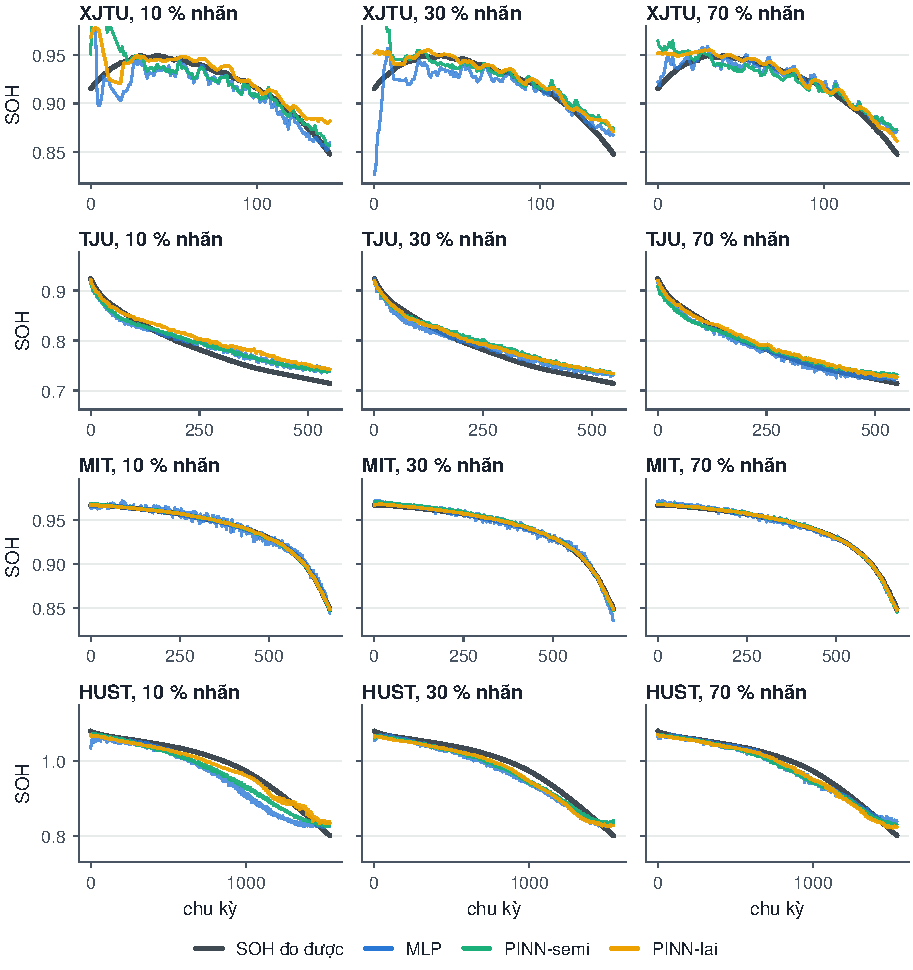
\includegraphics[width=0.92\textwidth]{graphics/fig_pred_traj.pdf}
\caption[Quỹ đạo SOH của cùng một cell kiểm tra mỗi bộ khi có 10, 30 và 70\,\% số cell mang nhãn]{Quỹ đạo SOH của cùng
một cell kiểm tra mỗi bộ khi có 10, 30 và 70\,\% số cell mang nhãn (lần lặp 0), dự đoán bởi MLP, PINN-semi và PINN-lai
(cấu hình cố định). Cell được chọn là cell có sai số MLP ở
trung vị của bộ tại 30\,\% nhãn, bỏ qua các cell có nhãn nhảy bất thường giữa hai chu kỳ; trục dọc theo dải SOH thực đo
nên vài chu kỳ đầu của XJTU vượt khỏi khung.}\label{fig:traj}
\end{figure}

\subsection{Lợi ích của PINN-semi đến từ đâu}\label{sec:source}

\begin{table}[!htbp]\centering\small
\caption[Tách nguồn gốc lợi ích ở 30\,\% nhãn]{Tách nguồn gốc lợi ích ở 30\,\% nhãn: MAE theo cell (×$10^{-3}$), trong ngoặc là tỉ số so với MLP.}\label{tab:source}
\begin{adjustbox}{max width=\textwidth}\begin{tabular}{lrrrr}\toprule
Mô hình (30\,\% nhãn) & XJTU & TJU & MIT & HUST \\\midrule
MLP & 15{,}95 & 11{,}33 & 3{,}40 & 19{,}80 \\
PINN-sup & 14{,}54 (0{,}91) & 10{,}67 (0{,}94) & 2{,}69 (0{,}79) & 17{,}82 (0{,}90) \\
chỉ đơn điệu & 14{,}13 (0{,}89) & 11{,}00 (0{,}97) & 2{,}86 (0{,}84) & 17{,}41 (0{,}88) \\
PINN-semi (Euler) & 13{,}37 (0{,}84) & 11{,}31 (1{,}00) & 3{,}01 (0{,}89) & 17{,}49 (0{,}88) \\
PINN hộp đen & 14{,}15 (0{,}89) & 10{,}91 (0{,}96) & 2{,}80 (0{,}83) & 17{,}49 (0{,}88) \\
PINN-semi & 13{,}44 (0{,}84) & 10{,}85 (0{,}96) & 2{,}58 (0{,}76) & 17{,}30 (0{,}87) \\
\bottomrule\end{tabular}\end{adjustbox}\end{table}


Bảng~\ref{tab:source} tách lợi ích ở 30\,\% nhãn. Chỉ riêng ràng buộc đơn điệu đã mang lại 62--95\,\% mức giảm sai số
(thang log) của PINN-semi so với MLP. Bỏ $\mathcal{L}_\text{ode}$ và $\mathcal{L}_\text{range}$ làm MAE bằng 1{,}01--1{,}11
lần PINN-semi đầy đủ, lớn nhất ở MIT. Ở 10\,\% nhãn, phần lợi ích do áp hàm mất mát vật lý lên cell không nhãn (PINN-semi
so với PINN-sup, tỉ số XJTU 0{,}74, TJU 0{,}94, MIT 0{,}62, HUST 0{,}73) chiếm 50--64\,\% mức giảm sai số so với MLP. Động học
xám tốt hơn động học hộp đen kiểu PINN4SOH có ý nghĩa thống kê ở 4 trong 16 trường hợp và kém hơn có ý nghĩa thống kê ở 1.
Ở 30\,\% nhãn, sai số của PINN hộp đen gần như trùng biến thể chỉ đơn điệu (chênh không quá 2\,\%). Điều này phù hợp với
giả thuyết rằng khi $G$ nhận cả $u_t$, mạng học được $G \approx u_t$ và phần dư động học được thoả mãn một cách tầm thường.
Vì sao phần vật lý đóng góp chủ yếu qua ràng buộc đơn điệu được phân tích ở \Cref{sec:vatly}.

\subsection{Mô hình chuỗi thời gian, GBDT và PINN-lai}\label{sec:e20res}

Bảng~\ref{tab:allmae} đặt bốn mô hình học sâu của đề cương cạnh GBDT, PINN-semi, PINN-lai và HiPINN-lai, cùng fold, cùng
cell có nhãn và 3 lần lặp.

\begin{table}[!htbp]\centering\footnotesize
\caption[MAE theo cell của mọi mô hình chính]{MAE theo cell ($\times10^{-3}$) trên tập kiểm tra của mọi mô hình chính, 3 lần lặp $\times$ 5 fold, cùng fold và cell có nhãn; in đậm là thấp nhất mỗi hàng. PINN-lai là cấu hình cố định ($\omega = \tfrac12$, $w = 10$), chốt trước khi đọc tập kiểm tra. HiPINN-lai là PINN-lai có thêm đặc trưng lịch sử của đặc trưng sạc ở những fold mà tập xác thực chọn; trên bộ không có dạng lịch sử nào được chọn (MIT), hai cột trùng nhau. HiPINN-lai là phân tích hậu kiểm (\Cref{sec:pinnlai}).}\label{tab:allmae}
\begin{adjustbox}{max width=\textwidth}\begin{tabular}{llrrrrrrrr}\toprule
 & & \multicolumn{8}{c}{MAE theo cell ($\times10^{-3}$) $\downarrow$} \\\cmidrule(lr){3-10}
Bộ & Nhãn & MLP & CNN & LSTM & Transformer & GBDT & PINN-semi & PINN-lai & HiPINN-lai \\\midrule
XJTU & 10\,\% & 23{,}27 & 16{,}01 & 16{,}62 & 17{,}63 & 14{,}01 & 14{,}65 & \textbf{12{,}83} & 13{,}34 \\
 & 30\,\% & 15{,}61 & 12{,}68 & 13{,}98 & 13{,}71 & \textbf{10{,}87} & 13{,}35 & 11{,}43 & 11{,}46 \\
 & 50\,\% & 14{,}10 & 11{,}69 & 11{,}98 & 12{,}05 & \textbf{10{,}18} & 13{,}20 & 10{,}65 & 10{,}63 \\
 & 70\,\% & 12{,}48 & 10{,}98 & 10{,}50 & 10{,}99 & \textbf{9{,}64} & 12{,}53 & 10{,}00 & 10{,}00 \\
TJU & 10\,\% & 15{,}81 & 14{,}22 & 13{,}08 & 14{,}14 & 12{,}60 & 14{,}01 & 11{,}79 & \textbf{11{,}73} \\
 & 30\,\% & 11{,}71 & 8{,}89 & 8{,}69 & 9{,}89 & \textbf{8{,}06} & 11{,}39 & 8{,}52 & 8{,}19 \\
 & 50\,\% & 9{,}96 & 7{,}31 & 7{,}24 & 9{,}31 & \textbf{7{,}17} & 10{,}74 & 7{,}77 & 7{,}36 \\
 & 70\,\% & 9{,}71 & 7{,}36 & 7{,}09 & 8{,}96 & \textbf{6{,}96} & 10{,}80 & 7{,}76 & 7{,}25 \\
MIT & 10\,\% & 9{,}02 & 3{,}30 & 3{,}26 & 3{,}87 & 3{,}15 & 3{,}29 & \textbf{2{,}52} & \textbf{2{,}52} \\
 & 30\,\% & 3{,}39 & 2{,}18 & 2{,}18 & 2{,}77 & 1{,}97 & 2{,}50 & \textbf{1{,}79} & \textbf{1{,}79} \\
 & 50\,\% & 3{,}06 & 1{,}99 & 2{,}04 & 2{,}71 & 1{,}74 & 2{,}45 & \textbf{1{,}67} & \textbf{1{,}67} \\
 & 70\,\% & 2{,}85 & 1{,}93 & 1{,}99 & 2{,}59 & \textbf{1{,}59} & 2{,}38 & \textbf{1{,}59} & \textbf{1{,}59} \\
HUST & 10\,\% & 41{,}62 & 22{,}77 & 24{,}51 & 21{,}95 & 23{,}84 & 22{,}76 & 20{,}52 & \textbf{20{,}08} \\
 & 30\,\% & 20{,}00 & 17{,}42 & 17{,}14 & 17{,}45 & 18{,}73 & 17{,}10 & 16{,}19 & \textbf{15{,}43} \\
 & 50\,\% & 18{,}13 & 15{,}04 & 15{,}52 & 16{,}00 & 15{,}82 & 16{,}42 & 14{,}29 & \textbf{13{,}24} \\
 & 70\,\% & 17{,}19 & 14{,}19 & 14{,}76 & 14{,}93 & 14{,}60 & 16{,}38 & 13{,}78 & \textbf{12{,}33} \\
\bottomrule\end{tabular}\end{adjustbox}\end{table}


So với MLP, tỉ số MAE của CNN là 0{,}37--0{,}90, của LSTM 0{,}36--0{,}90 và của Transformer 0{,}43--0{,}93. Mô hình chuỗi
thấp hơn MLP có ý nghĩa thống kê ở 42/48 phép so. Nhìn nhiều chu kỳ cho mô hình thấy xu thế của đặc trưng sạc và làm
trung bình nhiễu đo của từng chu kỳ. Trong ba mô hình chuỗi, LSTM thấp nhất ở 8/16 trường hợp. Mô hình chuỗi tốt nhất
thấp hơn GBDT ở 4/16 trường hợp (mọi mức nhãn trên HUST) và thấp hơn PINN-semi ở 14/16.

PINN-lai được xây dựng qua hai giai đoạn. Ở giai đoạn phát triển, chín hướng cải tiến được so trên tập xác thực của lần lặp 0, ở 10 và 50\,\% nhãn. Kết hợp với GBDT cho mức giảm lớn nhất (tỉ số trên tập xác thực so với PINN-semi 0{,}843 ở 10\,\% và 0{,}804 ở 50\,\% nhãn), còn nhóm ba mạng giảm vừa phải (0{,}963). Ba hướng làm sai số tăng là ràng buộc đơn điệu mạnh hơn (1{,}065), thêm phần dư Euler (1{,}289) và đặc trưng tương đối với mốc nhân quả (1{,}658). Cấu hình chốt là ba PINN-semi ghép với GBDT theo $\omega = \tfrac12$ rồi lọc xu thế với $w = 10$, ấn định trước khi đọc tập kiểm tra.

Trên tập kiểm tra, PINN-lai thấp hơn PINN-semi ở 16/16 trường hợp, trong đó 16 có ý nghĩa thống kê, với tỉ số 0{,}67--0{,}95. So với GBDT, PINN-lai thấp hơn ở 10/16 trường hợp (8 có ý nghĩa thống kê), và ở 10\,\% nhãn thấp hơn có ý nghĩa thống kê trên cả bốn bộ. GBDT chỉ còn tốt hơn có ý nghĩa thống kê ở TJU 70\,\%. Tính theo MAE trung bình ở \Cref{tab:allmae}, PINN-lai thấp hơn cả ba mô hình chuỗi ở 44/48 phép so. Các trường hợp mô hình chuỗi thấp hơn PINN-lai chỉ gồm CNN và LSTM ở TJU 50 và 70\,\%. Trên hai mức nhãn dùng khi phát triển, tỉ số trung bình nhân so với PINN-semi trên tập kiểm tra là 0{,}805, gần 0{,}823 trên tập xác thực, nên việc chọn trên tập xác thực không làm kết quả kiểm tra lạc quan đáng kể. Tính trung bình nhân trên 16 trường hợp, nhóm ba mạng đưa tỉ số so với PINN-semi xuống 0{,}961, kết hợp với GBDT xuống 0{,}798 và bộ lọc xuống 0{,}793. Bước kết hợp mang phần lớn lợi ích, vì lệch mức theo cell của nhóm PINN và của GBDT chỉ tương quan vừa (Pearson 0{,}50--0{,}80) và ngược dấu nhau ở 16--31\,\% số cell. Áp cùng công thức với ba MLP thay cho ba PINN-semi (MLP-lai), PINN-lai tốt hơn MLP-lai có ý nghĩa thống kê ở 7/16 trường hợp và kém hơn có ý nghĩa thống kê ở 1, với tỉ số trung bình nhân 0{,}716 ở 10\,\% và 1{,}002 ở 70\,\% nhãn. Phần vật lý vẫn đóng góp khi ít nhãn.

Sau khi có kết quả của bản cố định, đồ án thử thêm PINN-lai tinh chỉnh, chọn $(\omega, w)$ riêng trong từng fold chỉ bằng cell xác thực của fold đó (\Cref{sec:pinnlai}). Bản tinh chỉnh có MAE bằng 0{,}92--1{,}02 lần bản cố định, thấp hơn có ý nghĩa thống kê ở 5/16 và cao hơn có ý nghĩa thống kê ở 1/16 trường hợp. So với GBDT, bản tinh chỉnh thấp hơn ở 10/16 trường hợp (10 có ý nghĩa thống kê) và không cao hơn có ý nghĩa thống kê ở trường hợp nào. Mỗi fold chỉ có 6--13 cell xác thực nên cặp $(\omega, w)$ chọn được dao động giữa các fold. Bản tinh chỉnh là phân tích hậu kiểm và không được dùng ở các phần sau.


\begin{table}[!htbp]\centering\small
\caption[Thêm lịch sử của cell vào đầu vào]{MAE theo cell ($\times10^{-3}$) trên test khi thêm lịch sử của cell vào đầu vào, 3 lần lặp $\times$ 5 fold. Dạng lịch sử được chọn trên validation cho từng bộ và loại mô hình; trên MIT không dạng nào giảm sai số validation đủ 2\,\% nên không có cột lịch sử. PINN-lai là bản có trọng số ghép và cửa sổ lọc chọn trên validation. HiPINN-lai lấy cột PINN-lai có lịch sử ở những trường hợp validation chọn dùng lịch sử, còn lại lấy cột PINN-lai. $^{*}$/$^{\dagger}$: thấp hơn/cao hơn có ý nghĩa (Wilcoxon ghép cặp theo cell, $p < 0{,}05$) so với cột không lịch sử ngay trước.}\label{tab:hist}
\begin{tabular}{llrrrr}\toprule
 & & \multicolumn{2}{c}{PINN-semi} & \multicolumn{2}{c}{PINN-lai} \\\cmidrule(lr){3-4}\cmidrule(lr){5-6}
Bộ & Nhãn & không lịch sử & có lịch sử & không lịch sử & có lịch sử \\\midrule
XJTU & 10\,\% & 14{,}65 & 20{,}79$^{\dagger}$ & 12{,}71 & 15{,}95$^{\dagger}$ \\
 & 30\,\% & 13{,}35 & 15{,}34 & 10{,}78 & 11{,}25 \\
 & 50\,\% & 13{,}20 & 15{,}12 & 10{,}02 & 10{,}21 \\
 & 70\,\% & 12{,}53 & 13{,}17 & 9{,}50 & 9{,}73 \\
TJU & 10\,\% & 14{,}01 & 15{,}88$^{\dagger}$ & 11{,}70 & 11{,}83 \\
 & 30\,\% & 11{,}39 & 10{,}51$^{*}$ & 8{,}00 & 7{,}78$^{*}$ \\
 & 50\,\% & 10{,}74 & 9{,}43$^{*}$ & 7{,}23 & 6{,}92$^{*}$ \\
 & 70\,\% & 10{,}80 & 9{,}57$^{*}$ & 7{,}11 & 6{,}82$^{*}$ \\
MIT & 10\,\% & 3{,}29 & -- & 2{,}52 & -- \\
 & 30\,\% & 2{,}50 & -- & 1{,}75 & -- \\
 & 50\,\% & 2{,}45 & -- & 1{,}59 & -- \\
 & 70\,\% & 2{,}38 & -- & 1{,}48 & -- \\
HUST & 10\,\% & 22{,}76 & 23{,}63 & 20{,}36 & 20{,}15 \\
 & 30\,\% & 17{,}10 & 17{,}11 & 15{,}99 & 15{,}34$^{*}$ \\
 & 50\,\% & 16{,}42 & 14{,}81$^{*}$ & 14{,}26 & 13{,}17$^{*}$ \\
 & 70\,\% & 16{,}38 & 13{,}71$^{*}$ & 13{,}76 & 12{,}24$^{*}$ \\
\bottomrule\end{tabular}\end{table}

\paragraph{HiPINN-lai.} Bảng~\ref{tab:hist} cho sai số khi thêm lịch sử của cell vào đầu vào. Với PINN-lai, lịch sử giúp trên TJU và HUST khi có từ 30\,\% nhãn (MAE bằng 0{,}89--0{,}97 lần bản không lịch sử) nhưng làm kém đi trên XJTU (1{,}02--1{,}25 lần); ở 10\,\% nhãn, tỉ số là XJTU 1{,}25, TJU 1{,}01, HUST 0{,}99. Trên MIT không dạng lịch sử nào được validation chọn. HiPINN-lai chỉ dùng bản có lịch sử ở những trường hợp validation chọn (TJU và HUST từ 30\,\% nhãn) và trùng PINN-lai ở các trường hợp còn lại (\Cref{tab:allmae}).


Ở 30\,\% nhãn (Bảng~\ref{tab:allrm}), PINN-lai hoặc HiPINN-lai có RMSE hoặc MAPE thấp nhất ở 7/8 cột. Ở các cột còn lại, mô hình thấp nhất là GBDT. MLP có RMSE cao nhất trên cả bốn bộ. $R^2$ của PINN-lai ở 30\,\% nhãn, tính từ chu kỳ 10 của mỗi cell, là 0{,}867--0{,}992.


\begin{table}[!htbp]\centering\footnotesize
\caption[RMSE và MAPE của mọi mô hình chính ở 30\,\% nhãn]{Ở 30\,\% nhãn: RMSE theo cell ($\times10^{-3}$) và MAPE (\%, tính chung mọi chu kỳ) trên tập kiểm tra; in đậm là thấp nhất mỗi cột. PINN-lai và HiPINN-lai như ở Bảng~\ref{tab:allmae}.}\label{tab:allrm}
\begin{adjustbox}{max width=\textwidth}\begin{tabular}{lrrrrrrrr}\toprule
 & \multicolumn{2}{c}{XJTU} & \multicolumn{2}{c}{TJU} & \multicolumn{2}{c}{MIT} & \multicolumn{2}{c}{HUST} \\\cmidrule(lr){2-3}\cmidrule(lr){4-5}\cmidrule(lr){6-7}\cmidrule(lr){8-9}
Mô hình & RMSE $\downarrow$ & MAPE $\downarrow$ & RMSE $\downarrow$ & MAPE $\downarrow$ & RMSE $\downarrow$ & MAPE $\downarrow$ & RMSE $\downarrow$ & MAPE $\downarrow$ \\\midrule
MLP & 23{,}10 & 1{,}47 & 13{,}94 & 1{,}20 & 4{,}65 & 0{,}41 & 26{,}07 & 2{,}12 \\
CNN & 16{,}11 & 1{,}27 & 10{,}60 & 0{,}94 & 3{,}04 & 0{,}23 & 24{,}04 & 1{,}89 \\
LSTM & 17{,}91 & 1{,}32 & 10{,}27 & 0{,}94 & 3{,}05 & 0{,}23 & 23{,}45 & 1{,}85 \\
Transformer & 17{,}39 & 1{,}37 & 11{,}72 & 1{,}04 & 3{,}72 & 0{,}29 & 23{,}17 & 1{,}87 \\
GBDT & \textbf{14{,}37} & 1{,}19 & 9{,}74 & 0{,}90 & 2{,}93 & 0{,}21 & 25{,}98 & 2{,}04 \\
PINN-semi & 19{,}42 & 1{,}32 & 13{,}54 & 1{,}16 & 3{,}34 & 0{,}28 & 22{,}84 & 1{,}83 \\
PINN-lai & 15{,}80 & 1{,}18 & 10{,}14 & 0{,}91 & \textbf{2{,}46} & \textbf{0{,}19} & 22{,}29 & 1{,}75 \\
HiPINN-lai & 15{,}56 & \textbf{1{,}17} & \textbf{9{,}70} & \textbf{0{,}88} & \textbf{2{,}46} & \textbf{0{,}19} & \textbf{21{,}74} & \textbf{1{,}67} \\
\bottomrule\end{tabular}\end{adjustbox}\end{table}


\subsection{Khoảng dự đoán}\label{sec:conformal}

PINN-lai được gắn khoảng dự đoán 90\,\% bằng phương pháp conformal tách tập, hiệu chỉnh trên tập xác thực của từng fold.
Dạng thích nghi chia phần dư cho độ vênh giữa nhóm PINN và GBDT. Độ phủ thực tế trên tập kiểm tra là 84{,}9--92{,}6\,\% với
độ rộng cố định và 86{,}3--92{,}9\,\% với độ rộng thích nghi, trung bình 88{,}8\,\%. Độ rộng trung bình của dạng thích nghi
là 0{,}65--10{,}19\,\% SOH. Với độ rộng thích nghi, 14--25\,\% số cell có độ phủ dưới 80\,\%. Đó là các cell bị lệch mức
suốt cả đời.

\subsection{Ngân sách đo và cập nhật khi dùng}\label{sec:budgetres}

\begin{table}[!htbp]\centering\small
\caption[MAE theo cell theo ngân sách đo dung lượng]{MAE theo cell ($\times10^{-3}$) trên test, trung bình 3 lần lặp; trong ngoặc là phần trăm số chu kỳ của cell train có đo dung lượng (70\,\% số cell là toàn bộ). Hai cột đo thưa: mọi cell train được đo ở chu kỳ đầu, sau mỗi $qL$ chu kỳ và ở chu kỳ cuối. Cột cuối: đo thêm cell test theo cùng lịch, cập nhật bằng bộ lọc Kalman, sai số trên các chu kỳ không được đo. In đậm là thấp nhất trong năm cột đầu của mỗi hàng; cột cuối có đo thêm cell test nên không so cùng.}\label{tab:e28}
\begin{adjustbox}{max width=\textwidth}\begin{tabular}{lrrrrrr}\toprule
 & \multicolumn{6}{c}{MAE theo cell ($\times10^{-3}$) $\downarrow$} \\\cmidrule(lr){2-7}
Bộ & \begin{tabular}[b]{@{}r@{}}PINN-lai,\\30\,\% cell\end{tabular} & \begin{tabular}[b]{@{}r@{}}PINN-lai,\\70\,\% cell\end{tabular} & \begin{tabular}[b]{@{}r@{}}GBDT,\\70\,\% cell\end{tabular} & \begin{tabular}[b]{@{}r@{}}PINN-lai, đo\\mỗi $0{,}1L$\end{tabular} & \begin{tabular}[b]{@{}r@{}}PINN-lai, đo\\mỗi $0{,}05L$\end{tabular} & \begin{tabular}[b]{@{}r@{}}đo cả cell mới\\mỗi $0{,}1L$\end{tabular} \\\midrule
XJTU & 11{,}43 (44{,}1) & 10{,}00 & \textbf{9{,}64} & 10{,}51 (3{,}2) & 10{,}28 (6{,}0) & 7{,}46 \\
TJU & 8{,}52 (42{,}6) & 7{,}76 & \textbf{6{,}96} & 8{,}28 (3{,}1) & 7{,}54 (5{,}9) & 4{,}13 \\
MIT & 1{,}79 (42{,}7) & \textbf{1{,}59} & \textbf{1{,}59} & 1{,}91 (1{,}9) & 1{,}67 (3{,}6) & 1{,}18 \\
HUST & 16{,}19 (43{,}1) & \textbf{13{,}78} & 14{,}60 & 13{,}87 (0{,}6) & \textbf{13{,}78} (1{,}2) & 5{,}00 \\
\bottomrule\end{tabular}\end{adjustbox}\end{table}


\begin{figure}[!htbp]\centering
% Hình chép từ báo cáo đã nộp (không còn dữ liệu để vẽ lại); nhãn trục hoành "cell train" được viết lại bằng tiếng
% Việt: ô trắng phủ đúng dòng nhãn cũ (toạ độ lấy bằng pdftotext -bbox, đơn vị là phần của khung hình) và nhãn mới
% cùng phông TeX Gyre Heros.
\begin{tikzpicture}
\node[anchor=south west, inner sep=0] (img) at (0,0) {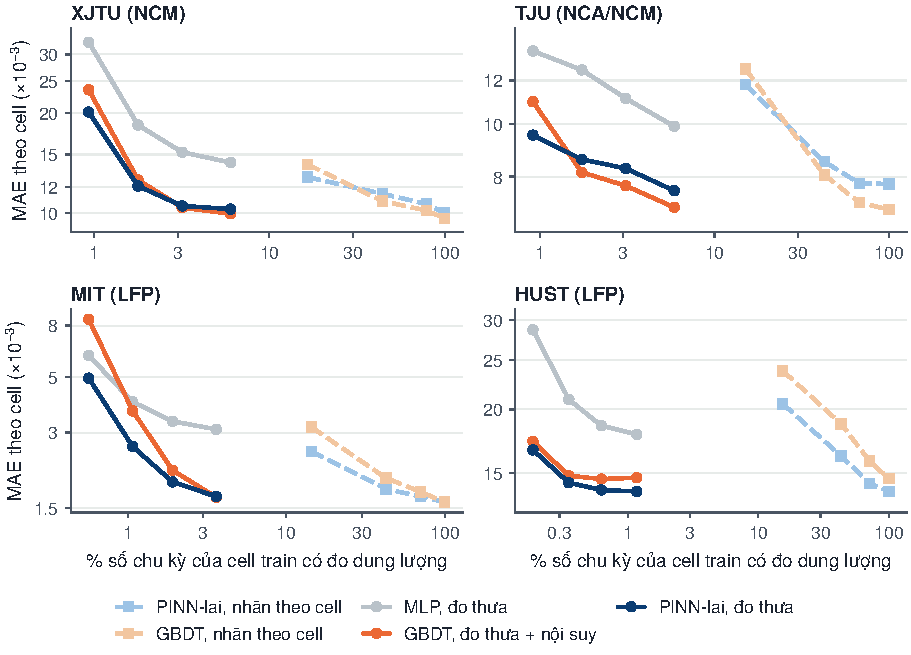
\includegraphics[width=\textwidth]{graphics/fig_e28_budget.pdf}};
\begin{scope}[x={(img.south east)}, y={(img.north west)}]
\fill[white] (0.0926, 0.1220) rectangle (0.4927, 0.1678);
\fill[white] (0.5803, 0.1220) rectangle (0.9800, 0.1678);
\node[inner sep=0, font=\fontsize{8.4}{10}\fontfamily{qhv}\selectfont] at (0.2927, 0.1460)
  {\% số chu kỳ của cell huấn luyện có đo dung lượng};
\node[inner sep=0, font=\fontsize{8.4}{10}\fontfamily{qhv}\selectfont] at (0.7802, 0.1460)
  {\% số chu kỳ của cell huấn luyện có đo dung lượng};
\end{scope}
\end{tikzpicture}
\caption[MAE theo phần trăm số chu kỳ của cell huấn luyện có đo dung lượng]{MAE theo cell trên tập kiểm tra theo phần trăm
số chu kỳ của cell huấn luyện có đo dung lượng (hai trục thang log). Nét đứt: nhãn theo cell (10, 30, 50, 70\,\% số cell
có nhãn đầy đủ); nét liền: đo thưa mọi cell huấn luyện theo lịch $qL$, $q$ = 0{,}5; 0{,}2; 0{,}1; 0{,}05.}\label{fig:e28}
\end{figure}

Gắn nhãn đầy đủ cho 30\,\% số cell tương ứng 43--44\,\% số chu kỳ huấn luyện. Đo mỗi $0{,}05L$ chu kỳ trên mọi cell chỉ
dùng 1{,}2--6{,}0\,\% số chu kỳ, ít hơn 7--37 lần, nhưng PINN-lai học theo cách này có MAE bằng 0{,}85--0{,}93 lần PINN-lai
học với 30\,\% số cell, thấp hơn có ý nghĩa thống kê trên cả bốn bộ (Bảng~\ref{tab:e28}, Hình~\ref{fig:e28}). So với 70\,\%
số cell, tỉ số là 0{,}97--1{,}05: tốt hơn có ý nghĩa thống kê ở TJU và kém hơn có ý nghĩa thống kê ở MIT. Lý do là phần lớn
sai số là lệch mức riêng của từng cell, mô hình chỉ học được khi thấy nhãn của chính cell đó, còn các chu kỳ liền nhau của
một cell gần như lặp lại thông tin của nhau.

Khi cell mới cũng được đo theo lịch $0{,}1L$ (1--3\,\% số chu kỳ của nó) và ước lượng của PINN-lai được cập nhật bằng bộ lọc Kalman, MAE trên các chu kỳ không được đo còn 1{,}0--7{,}4 ($\times10^{-3}$), bằng 0{,}35--0{,}76 lần GBDT học với 70\,\% số cell có nhãn đầy đủ nhưng không đo cell mới (cột cuối của Bảng~\ref{tab:e28}). GBDT-cập nhật, mô hình học thẳng thay đổi SOH kể từ lần đo gần nhất, thấp hơn bộ lọc Kalman ở 48/48 trường hợp bộ $\times$ mức nhãn $\times$ lịch đo (tỉ số 0{,}14--0{,}98) và thấp hơn việc giữ nguyên giá trị đo gần nhất ở 48/48 trường hợp (tỉ số 0{,}07--0{,}52). Trong cả hai cách, lịch đo của cell kiểm tra dùng thang đời $L$ tính trên cell huấn luyện của fold.


\label{sec:anchor}Đồ án đưa đặc trưng lịch sử của HiGBDT vào bài toán cập nhật của \Cref{sec:mo_rong}: ước lượng SOH ở các chu kỳ không đo từ lần đo dung lượng gần nhất, trên cùng fold với các thí nghiệm khác, 30\,\% nhãn, $L$ và chuẩn hoá tính trên cell huấn luyện. GBDT-cập nhật dùng đặc trưng sạc hiện tại và độ đổi của chúng kể từ lần đo, SOH ở lần đo, khoảng chu kỳ tới lần đo và độ dốc giữa hai lần đo gần nhất. Hai mô hình dùng lịch sử thêm hai trung bình trượt mũ nhân quả của đặc trưng sạc ($\rho = 0{,}1$ và $0{,}03$), log khoảng chu kỳ và chỉ số chu kỳ: HiGBDT-$\Delta$ học độ giảm SOH kể từ lần đo, HiGBDT-R học phần dư so với ngoại suy tuyến tính từ hai lần đo gần nhất. HiGBDT-V chọn trên tập xác thực, theo từng lịch đo, một trong ba mô hình đó và trọng số trộn nó với giữ lần đo hoặc ngoại suy tuyến tính. Mỗi mô hình học trên tối đa khoảng 60 nghìn cặp (chu kỳ, lần đo), cân theo cell và lịch đo, có thêm hai pha đo ngẫu nhiên cho mỗi lịch thưa. Số cây chọn trên tập xác thực. \Cref{tab:anchor} cho kết quả. Chỉ với một lần đo mỗi $0{,}2L$ chu kỳ, GBDT-cập nhật đạt MAE 1{,}27--6{,}12 ($\times10^{-3}$), bằng 0{,}10--0{,}30 lần việc giữ nguyên giá trị đo gần nhất. Khi biết mọi lần đo trước, HiGBDT-R có MAE bằng 0{,}57--0{,}95 lần GBDT-cập nhật. Khi đo thưa, lịch sử không giúp: HiGBDT-V chỉ có MAE trung bình thấp hơn GBDT-cập nhật ở 1/4 bộ với lịch đo mỗi $0{,}2L$ và 1/4 bộ với lịch mỗi $0{,}1L$, và kém hơn có ý nghĩa thống kê trên TJU ở cả ba lịch đo thưa. Lịch sử có lợi hơn khi đo dày: 1/4 bộ (HUST) ở lịch mỗi $0{,}05L$ và 4/4 bộ khi biết mọi lần đo trước, nhưng mức sau không phải là đo thưa. Ở MIT với lịch mỗi $0{,}05L$ và mỗi $0{,}1L$, HiGBDT-V tốt hơn ở 75/125 và 68/125 cell nên kiểm định nghiêng về nó, dù MAE trung bình cao hơn vì một cell sai lớn. Vì vậy đồ án giữ GBDT-cập nhật cho lịch đo thưa. \Cref{fig:e34cost} đặt sai số cạnh số lần đo dung lượng trung bình mỗi cell. Với lịch mỗi $0{,}2L$, GBDT-cập nhật có MAE thấp hơn việc giữ lần đo với lịch mỗi $0{,}05L$ trên cả bốn bộ, tức với số lần đo ít hơn 3{,}7--3{,}8 lần.

\begin{table}[!htbp]\centering\small
\caption[HiGBDT cho bài toán cập nhật]{Cập nhật SOH ở các chu kỳ không đo từ lần đo dung lượng gần nhất, theo lịch đo: MAE theo cell ($\times10^{-3}$), 30\,\% nhãn, 3 lần lặp $\times$ 5 fold. $^{*}$/$^{\dagger}$: HiGBDT-V tốt hơn/kém hơn có ý nghĩa thống kê so với GBDT-cập nhật (Wilcoxon ghép cặp theo cell, hiệu chỉnh Holm qua bốn bộ trong từng lịch đo, $p<0{,}05$).}\label{tab:anchor}
\begin{adjustbox}{max width=\textwidth}\begin{tabular}{lrrrrrr}\toprule
 & \multicolumn{6}{c}{MAE của SOH cập nhật ($\times10^{-3}$) $\downarrow$} \\\cmidrule(lr){2-7}
Bộ & \begin{tabular}[b]{@{}r@{}}Giữ\\lần đo\end{tabular} & \begin{tabular}[b]{@{}r@{}}Tuyến\\tính\end{tabular} & \begin{tabular}[b]{@{}r@{}}GBDT-\\cập nhật\end{tabular} & \begin{tabular}[b]{@{}r@{}}\\HiGBDT-$\Delta$\end{tabular} & \begin{tabular}[b]{@{}r@{}}\\HiGBDT-R\end{tabular} & \begin{tabular}[b]{@{}r@{}}\\HiGBDT-V\end{tabular} \\\midrule
\multicolumn{7}{@{}l}{\textit{lịch đo mỗi $0{,}2L$}} \\
XJTU & 20{,}24 & 16{,}99 & \textbf{6{,}12} & 6{,}29 & 6{,}58 & 6{,}25\phantom{$^{*}$} \\
TJU & 20{,}73 & 14{,}23 & \textbf{2{,}77} & 3{,}10 & 3{,}94 & 2{,}90$^{\dagger}$ \\
MIT & 10{,}54 & 6{,}63 & 1{,}27 & \textbf{1{,}26} & 1{,}57 & 1{,}27\phantom{$^{*}$} \\
HUST & 24{,}99 & 9{,}73 & 2{,}56 & \textbf{2{,}47} & 2{,}63 & 2{,}51\phantom{$^{*}$} \\
\addlinespace[3pt]
\multicolumn{7}{@{}l}{\textit{lịch đo mỗi $0{,}1L$}} \\
XJTU & 11{,}79 & 8{,}81 & \textbf{3{,}82} & 4{,}21 & 4{,}21 & 3{,}91\phantom{$^{*}$} \\
TJU & 12{,}66 & 8{,}12 & \textbf{1{,}87} & 2{,}06 & 2{,}23 & 2{,}21$^{\dagger}$ \\
MIT & 6{,}46 & 3{,}23 & \textbf{0{,}91} & 0{,}93 & 0{,}97 & 0{,}92$^{*}$ \\
HUST & 13{,}35 & 3{,}19 & 1{,}09 & \textbf{1{,}07} & 1{,}07 & 1{,}09\phantom{$^{*}$} \\
\addlinespace[3pt]
\multicolumn{7}{@{}l}{\textit{lịch đo mỗi $0{,}05L$}} \\
XJTU & 6{,}45 & 4{,}87 & \textbf{2{,}63} & 2{,}96 & 2{,}86 & 2{,}69\phantom{$^{*}$} \\
TJU & 6{,}57 & 3{,}93 & \textbf{1{,}11} & 1{,}23 & 1{,}29 & 1{,}19$^{\dagger}$ \\
MIT & 3{,}65 & 1{,}61 & \textbf{0{,}67} & 0{,}73 & 0{,}71 & 0{,}68$^{*}$ \\
HUST & 6{,}93 & 1{,}05 & 0{,}55 & 0{,}55 & \textbf{0{,}52} & 0{,}54\phantom{$^{*}$} \\
\addlinespace[3pt]
\multicolumn{7}{@{}l}{\textit{biết mọi lần đo trước}} \\
XJTU & 1{,}74 & 1{,}55 & 1{,}31 & 1{,}46 & \textbf{1{,}24} & 1{,}25$^{*}$ \\
TJU & 0{,}93 & 0{,}65 & 0{,}32 & 0{,}35 & \textbf{0{,}31} & 0{,}31$^{*}$ \\
MIT & 0{,}42 & 0{,}37 & 0{,}40 & 0{,}39 & \textbf{0{,}32} & 0{,}33$^{*}$ \\
HUST & 0{,}19 & 0{,}29 & 0{,}12 & 0{,}15 & \textbf{0{,}07} & \textbf{0{,}07}$^{*}$ \\
\bottomrule\end{tabular}\end{adjustbox}\end{table}

\begin{figure}[!htbp]\centering
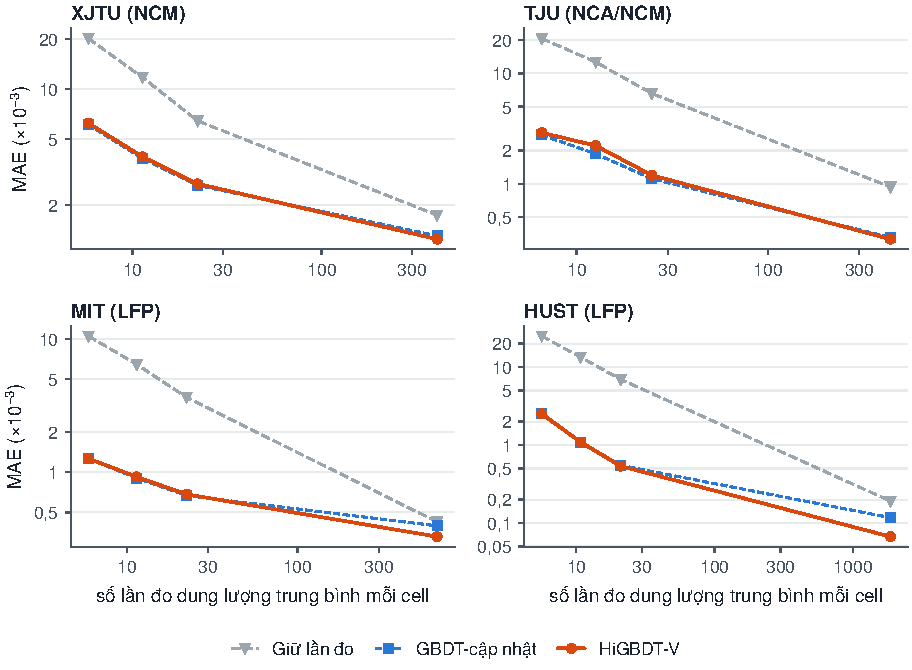
\includegraphics[width=\textwidth]{graphics/fig_e34_cost.pdf}
\caption[Sai số cập nhật theo số lần đo]{MAE ($\times10^{-3}$, thang log) của SOH cập nhật theo số lần đo dung lượng trung bình mỗi cell, bốn lịch đo (mỗi $0{,}2L$, $0{,}1L$, $0{,}05L$ và biết mọi lần đo trước), 30\,\% nhãn, trung bình qua 3 lần lặp. Đường nối chỉ để dễ so, không phải quan hệ liên tục đã ước lượng.}\label{fig:e34cost}
\end{figure}


\FloatBarrier
\subsection{Dự báo SOH, dung lượng và RUL: HiGBDT và HiPINN}\label{sec:e33res}

\Cref{tab:e33} cho MAE của SOH dự báo ở hai ngân sách nhãn, 30\,\% nhãn hoặc mọi cell huấn luyện. Lịch sử SOH của cell kiểm tra tới gốc là dung lượng đo. Hai mô hình chỉ dựa vào chính cell là giữ nguyên và ngoại suy tuyến tính có sai số gấp 1{,}8--10{,}3 lần HiPINN nên không đưa vào bảng (có trong \Cref{fig:e33mae}).

\begin{table}[!htbp]\centering\small
\caption[MAE của SOH dự báo theo mô hình]{MAE theo cell ($\times10^{-3}$) của SOH dự báo trên mọi chu kỳ đo được sau gốc ($0{,}2L$, $0{,}4L$, $0{,}6L$), trung bình qua 3 lần lặp; in đậm là thấp nhất mỗi hàng. $^{*}$/$^{\dagger}$: HiPINN tốt hơn/kém hơn có ý nghĩa thống kê so với HiGBDT theo kiểm định Wilcoxon ghép cặp theo cell (Holm qua bốn bộ, $p<0{,}05$).}\label{tab:e33}
\begin{adjustbox}{max width=\textwidth}\begin{tabular}{lrrrrrrrr}\toprule
 & \multicolumn{8}{c}{MAE của SOH dự báo ($\times10^{-3}$) $\downarrow$} \\\cmidrule(lr){2-9}
 & \multicolumn{3}{c}{chỉ đặc trưng gốc} & \multicolumn{5}{c}{có đặc trưng lịch sử} \\\cmidrule(lr){2-4}\cmidrule(lr){5-9}
Bộ & \begin{tabular}[b]{@{}r@{}}GBDT\\theo tầm\end{tabular} & \begin{tabular}[b]{@{}r@{}}PINN-\\dự báo\end{tabular} & \begin{tabular}[b]{@{}r@{}}PINN-\\GBDT\end{tabular} & \begin{tabular}[b]{@{}r@{}}\\HiGBDT\end{tabular} & \begin{tabular}[b]{@{}r@{}}PINN có\\lịch sử\end{tabular} & \begin{tabular}[b]{@{}r@{}}Theo\\đời\end{tabular} & \begin{tabular}[b]{@{}r@{}}\\HiPINN-w\end{tabular} & \begin{tabular}[b]{@{}r@{}}\\HiPINN\end{tabular} \\\midrule
\multicolumn{9}{@{}l}{\textit{30\,\% nhãn}} \\
XJTU & 18{,}71 & 31{,}23 & 26{,}51 & 17{,}34 & 27{,}25 & 19{,}54 & 25{,}26 & \textbf{16{,}37}\phantom{$^{*}$} \\
TJU & 7{,}55 & 9{,}66 & 9{,}01 & 7{,}07 & 9{,}03 & 8{,}91 & 8{,}05 & \textbf{6{,}10}$^{*}$ \\
MIT & 12{,}07 & 16{,}72 & 14{,}47 & \textbf{10{,}24} & 18{,}27 & 12{,}72 & 12{,}00 & 10{,}29\phantom{$^{*}$} \\
HUST & 14{,}13 & 18{,}88 & 15{,}82 & 12{,}78 & 16{,}41 & 12{,}84 & 13{,}90 & \textbf{12{,}27}$^{*}$ \\
\addlinespace[3pt]
\multicolumn{9}{@{}l}{\textit{mọi cell huấn luyện}} \\
XJTU & 15{,}81 & 15{,}15 & 14{,}49 & 13{,}97 & 16{,}79 & 15{,}59 & 15{,}42 & \textbf{13{,}21}$^{*}$ \\
TJU & 6{,}30 & 7{,}44 & 6{,}99 & 5{,}89 & 7{,}08 & 7{,}00 & 6{,}84 & \textbf{5{,}09}$^{*}$ \\
MIT & 10{,}82 & 13{,}15 & 11{,}66 & 9{,}43 & 13{,}78 & 11{,}20 & 9{,}93 & \textbf{9{,}27}$^{*}$ \\
HUST & 12{,}17 & 13{,}61 & 11{,}79 & 11{,}24 & 12{,}54 & 11{,}24 & 10{,}90 & \textbf{10{,}35}$^{*}$ \\
\bottomrule\end{tabular}\end{adjustbox}\end{table}

Trước hết, xét tác động của việc thêm lịch sử vào từng nhánh. Với GBDT, đặc trưng lịch sử giúp rõ rệt: HiGBDT có MAE bằng 0{,}85--0{,}94 lần GBDT theo tầm, thấp hơn có ý nghĩa thống kê ở cả hai ngân sách trên cả bốn bộ. Cây quyết định dùng được trực tiếp những thông tin như độ dốc trên nhiều cửa sổ hay mức dao động gần đây để nhận ra cell đang suy giảm nhanh hay chậm. Với PINN-dự báo, lợi ích không đều: bản có lịch sử có MAE bằng 0{,}87--1{,}11 lần bản không có lịch sử, thấp hơn có ý nghĩa thống kê ở cả hai ngân sách trên HUST. Một cách giải thích: mạng chỉ chọn hai tham số $(a, \lambda)$ của một đường suy giảm có dạng cố định, nên thông tin thêm từ lịch sử chủ yếu giúp ước lượng tốc độ hiện tại, điều mà hai độ dốc trong $\mathbf{z}_k$ đã có một phần, trong khi số đầu vào tăng hơn gấp đôi. Vì vậy HiPINN giữ PINN-dự báo không có lịch sử làm nhánh PINN, còn lịch sử được đưa vào mô hình qua hai nhánh kia.

HiPINN-w, phương án đầu của HiPINN, chọn trọng số của ba nhánh và nhánh PINN trên nửa tập xác thực dùng để chọn. Nửa này chỉ có 3--7 cell mỗi lượt. Trên chính nửa đó (\Cref{tab:e33val}), HiPINN-w có MAE bằng 0{,}71--0{,}92 lần HiGBDT. Trên nửa hiệu chỉnh, tỉ số này là 0{,}80--1{,}45, và trên cell kiểm tra là 0{,}97--1{,}46, cao hơn HiGBDT ở 7/8 trường hợp. Trọng số chọn trên vài cell phản ánh chính các cell đó nhiều hơn là quy luật chung, nên ưu thế mất đi khi chuyển sang cell khác. HiPINN vì vậy dùng trung vị, không có trọng số cần chọn (\Cref{sec:e33pp}).

Xét tiếp HiPINN, mô hình lấy trung vị của ba nhánh. HiPINN có MAE thấp nhất trong tám mô hình của \Cref{tab:e33} ở 7/8 trường hợp (bộ $\times$ ngân sách). So với HiGBDT, nhánh tốt nhất khi đứng riêng, MAE của HiPINN bằng 0{,}86--1{,}01 lần và thấp hơn ở 7/8 trường hợp. Theo kiểm định ghép cặp, HiPINN tốt hơn có ý nghĩa thống kê ở 6/8 và kém hơn có ý nghĩa thống kê ở 0/8 trường hợp, với 62--82\,\% số cell có sai số thấp hơn. So với PINN-GBDT, MAE của HiPINN bằng 0{,}62--0{,}91 lần (thấp hơn có ý nghĩa thống kê ở 8/8 trường hợp). Trung vị cũng tốt hơn hai cách ghép còn lại: MAE của HiPINN bằng 0{,}65--0{,}95 lần HiPINN-w (thấp hơn ở 8/8 trường hợp) và 0{,}79--0{,}99 lần HiPINN-tb, tức trung bình đều ba nhánh (thấp hơn ở 8/8). Khi một nhánh sai xa, trung bình bị kéo theo, còn trung vị đi theo hai nhánh còn lại.

Dạng trung vị được chọn sau khi đã thấy kết quả kiểm tra của HiPINN-w, nên cần một kiểm tra không dùng cell kiểm tra. Nửa hiệu chỉnh không dùng để chọn gì cho các mô hình HiGBDT, HiPINN-w, HiPINN-tb và HiPINN, và sai số của trung vị trên nửa này chưa được xem khi quyết định. Trên nửa này (\Cref{tab:e33val}), HiPINN có MAE thấp hơn HiPINN-w ở 7/8 trường hợp. So với HiGBDT, HiPINN thấp hơn ở 4/4 bộ khi học trên mọi cell huấn luyện (tốt hơn có ý nghĩa thống kê ở 3) và 2/4 bộ với 30\,\% nhãn. Kết quả cùng chiều với tập kiểm tra khi học trên mọi cell huấn luyện. Với 30\,\% nhãn, ưu thế của HiPINN so với HiGBDT trên tập kiểm tra chưa được nửa hiệu chỉnh xác nhận, nên một phần ưu thế đó có thể do chính việc chọn dạng trung vị sau khi xem kết quả.

\begin{table}[!htbp]\centering\small
\caption[MAE của SOH dự báo trên hai nửa tập xác thực]{MAE theo cell ($\times10^{-3}$) của SOH dự báo trên hai nửa tập xác thực; mỗi cell lấy trung bình qua các lượt mà nó thuộc nửa đó. Nửa chọn là nơi chọn trọng số của HiPINN-w; nửa hiệu chỉnh không dùng để chọn gì cho các mô hình trong bảng. In đậm là thấp nhất trong mỗi nửa. $^{*}$/$^{\dagger}$: trên nửa hiệu chỉnh, HiPINN tốt hơn/kém hơn có ý nghĩa thống kê so với HiGBDT (Wilcoxon ghép cặp theo cell, Holm qua bốn bộ, $p<0{,}05$).}\label{tab:e33val}
\begin{adjustbox}{max width=\textwidth}\begin{tabular}{lrrrrrrr}\toprule
 & \multicolumn{7}{c}{MAE theo cell ($\times10^{-3}$) $\downarrow$} \\\cmidrule(lr){2-8}
 & \multicolumn{3}{c}{nửa chọn} & \multicolumn{4}{c}{nửa hiệu chỉnh} \\\cmidrule(lr){2-4}\cmidrule(lr){5-8}
Bộ & \begin{tabular}[b]{@{}r@{}}\\HiGBDT\end{tabular} & \begin{tabular}[b]{@{}r@{}}\\HiPINN-w\end{tabular} & \begin{tabular}[b]{@{}r@{}}\\HiPINN\end{tabular} & \begin{tabular}[b]{@{}r@{}}\\HiGBDT\end{tabular} & \begin{tabular}[b]{@{}r@{}}\\HiPINN-w\end{tabular} & \begin{tabular}[b]{@{}r@{}}\\HiPINN-tb\end{tabular} & \begin{tabular}[b]{@{}r@{}}\\HiPINN\end{tabular} \\\midrule
\multicolumn{8}{@{}l}{\textit{30\,\% nhãn}} \\
XJTU & 13{,}07 & \textbf{10{,}64} & 12{,}49 & \textbf{16{,}56} & 23{,}94 & 18{,}70 & 16{,}79\phantom{$^{*}$} \\
TJU & 6{,}95 & \textbf{5{,}53} & 6{,}18 & 6{,}61 & \textbf{5{,}29} & 6{,}55 & 5{,}79\phantom{$^{*}$} \\
MIT & 8{,}88 & \textbf{8{,}19} & 8{,}71 & \textbf{9{,}93} & 12{,}45 & 11{,}86 & 10{,}39\phantom{$^{*}$} \\
HUST & 11{,}35 & \textbf{10{,}03} & 11{,}45 & 12{,}30 & 13{,}06 & 13{,}18 & \textbf{12{,}26}\phantom{$^{*}$} \\
\addlinespace[3pt]
\multicolumn{8}{@{}l}{\textit{mọi cell huấn luyện}} \\
XJTU & 12{,}37 & \textbf{10{,}15} & 11{,}46 & 13{,}77 & 15{,}95 & 13{,}23 & \textbf{12{,}91}$^{*}$ \\
TJU & 6{,}36 & \textbf{4{,}51} & 5{,}35 & 6{,}06 & 5{,}18 & 5{,}35 & \textbf{5{,}07}$^{*}$ \\
MIT & 8{,}26 & \textbf{7{,}58} & 8{,}08 & 9{,}09 & 9{,}98 & 10{,}59 & \textbf{8{,}87}\phantom{$^{*}$} \\
HUST & 10{,}54 & \textbf{8{,}67} & 9{,}80 & 11{,}53 & 11{,}22 & 10{,}89 & \textbf{10{,}75}$^{*}$ \\
\bottomrule\end{tabular}\end{adjustbox}\end{table}

\begin{figure}[!htbp]\centering
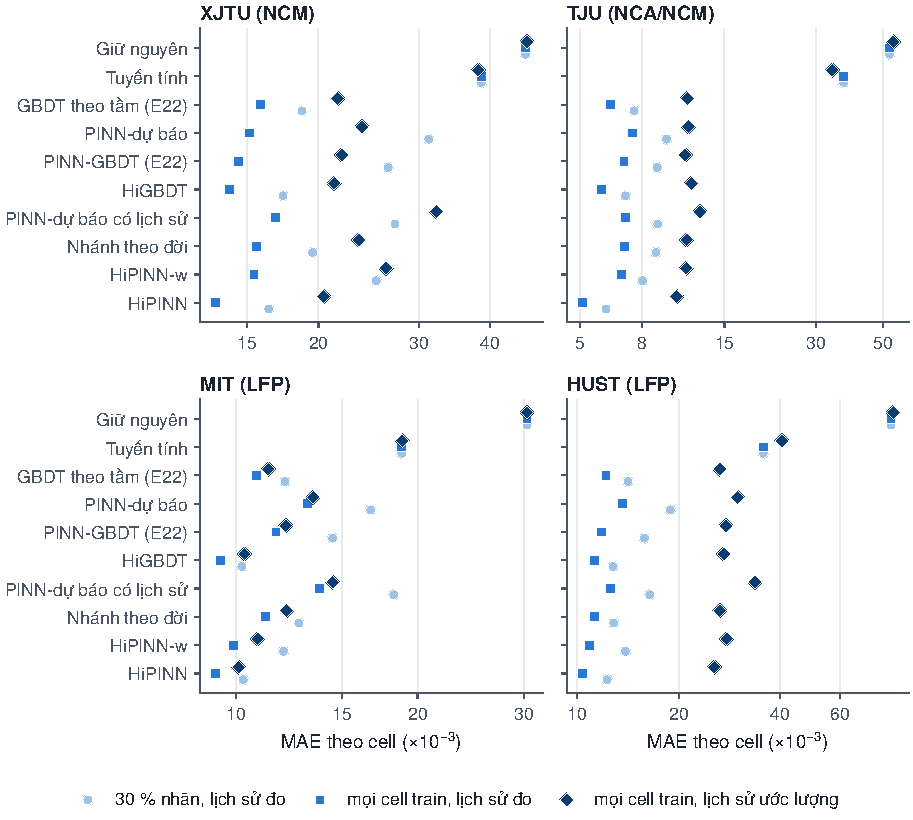
\includegraphics[width=\textwidth]{graphics/fig_e33_mae.pdf}
\caption[MAE của SOH dự báo theo mô hình và ngân sách nhãn]{MAE theo cell (trung bình qua 3 lần lặp, thang log) của các mô hình ở hai ngân sách nhãn, 30\,\% nhãn hoặc mọi cell huấn luyện; lịch sử SOH tới gốc là dung lượng đo.}\label{fig:e33mae}
\end{figure}

Sai số dự báo không đều theo tuổi của cell. \Cref{fig:e33tail} chia sai số theo phần đời của chính cell (mọi cell huấn luyện, lịch sử đo). Sai số của các mô hình nhìn chung tăng về cuối đời, và với HiPINN lớn nhất ở 10\,\% đời cuối trên cả bốn bộ. Ở MIT, MAE trên 10\,\% đời cuối là 26{,}2 với PINN-GBDT và 20{,}6 với HiPINN, giảm 22\,\% ($\times10^{-3}$; HiGBDT 20{,}8). Phần sai số còn lại chủ yếu là dự báo cao hơn thực tế: độ lệch trung bình ở đoạn này là +12{,}7 với HiPINN và +15{,}3 với HiGBDT. Thời điểm gãy mỗi cell một khác, nên dự báo trực tiếp thành một đường trung bình thoải hơn thực tế. Nhánh theo đời đặt hình dạng suy giảm lên đời dự đoán của từng cell nên độ lệch chỉ còn +3{,}6, nhưng MAE của nó (21{,}7) không thấp hơn vì khi đời bị đoán sai thì điểm gãy cũng bị đặt sai chỗ. Ở đoạn này, GBDT theo tầm có MAE thấp nhất (19{,}2). Trên bốn bộ, MAE ở 10\,\% đời cuối của HiPINN thấp hơn PINN-GBDT ở 4/4 bộ với mọi cell huấn luyện và 4/4 bộ với 30\,\% nhãn.

\begin{figure}[!htbp]\centering
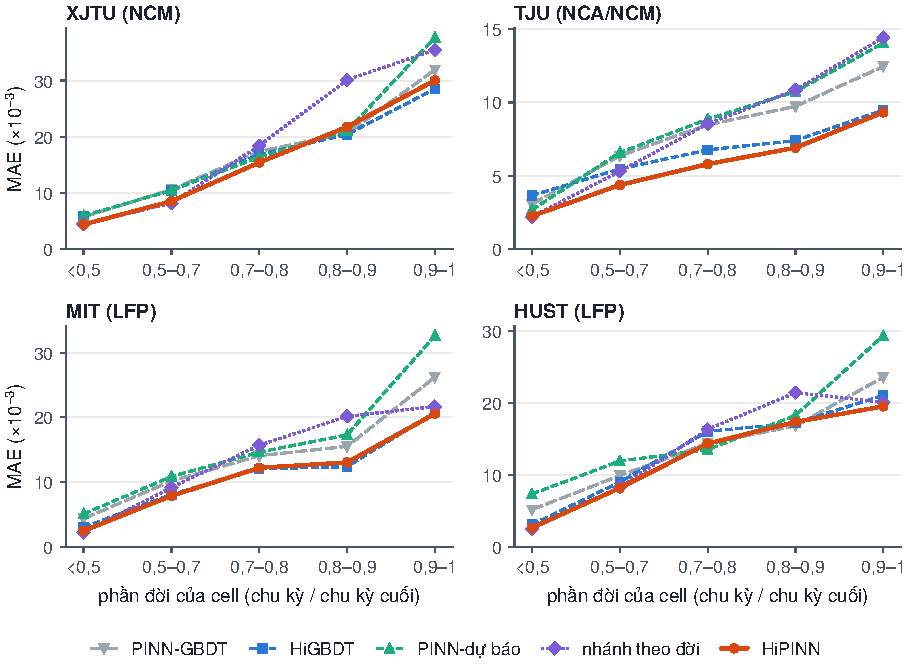
\includegraphics[width=\textwidth]{graphics/fig_e33_tail.pdf}
\caption[Sai số dự báo theo phần đời của cell]{MAE ($\times10^{-3}$) của SOH dự báo theo phần đời của chính cell (chu kỳ chia chu kỳ cuối ghi được), mọi cell huấn luyện, lịch sử đo, trung bình theo cell. Phần đời chỉ dùng để chia nhóm khi chấm, mô hình không biết nó.}\label{fig:e33tail}
\end{figure}

\Cref{fig:e33traj} minh hoạ dự báo cho một cell mỗi bộ. Ở mỗi tầm, HiPINN trùng với nhánh nằm giữa trong ba nhánh, nên đường của nó gãy khúc ở chỗ hai nhánh cắt nhau. Hình chỉ vẽ hai nhánh có đặc trưng lịch sử. Ở những đoạn HiPINN không trùng đường nào trong hai đường đó, nhánh nằm giữa là PINN-dự báo.

\begin{figure}[!htbp]\centering
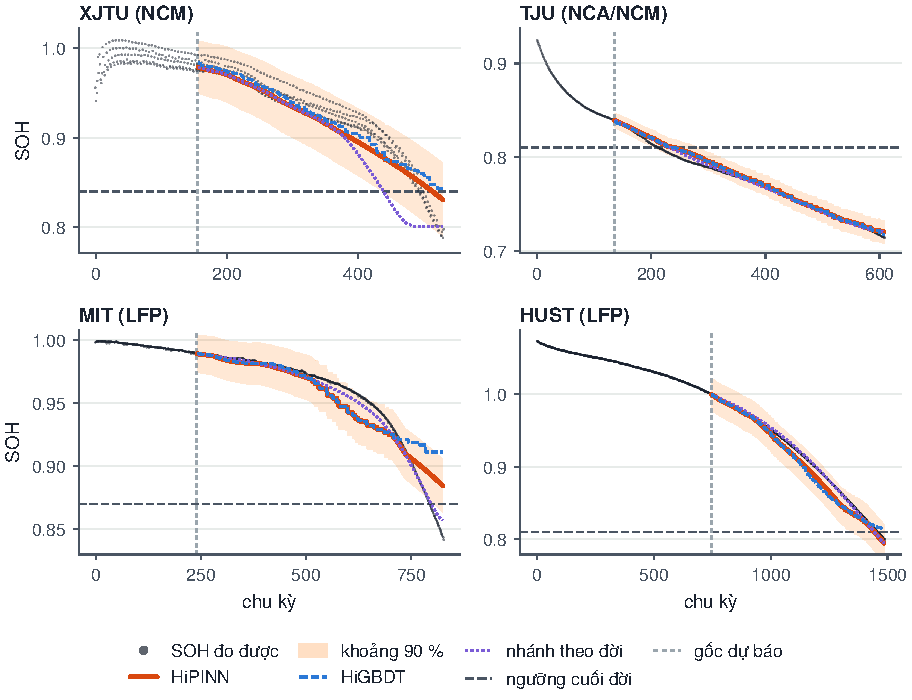
\includegraphics[width=\textwidth]{graphics/fig_e33_traj.pdf}
\caption[Dự báo của HiPINN so với SOH đo được]{Dự báo của HiPINN, HiGBDT và nhánh theo đời so với SOH đo được cho một cell kiểm tra mỗi bộ: mọi cell huấn luyện, lịch sử đo, lần lặp 0, gốc ở $0{,}4L$; trong các cell còn ít nhất $0{,}25L$ chu kỳ đo sau gốc, chọn cell có sai số của HiPINN ở trung vị. Khoảng 90\,\% tính bằng phương pháp conformal. PINN-dự báo, nhánh thứ ba của HiPINN, không vẽ để hình dễ đọc. Ở XJTU, cell được chọn thuộc nhóm R2.5, nhóm có chế độ xả thay đổi. Dung lượng đo của cell này lặp lại theo vòng 5 chu kỳ: chênh lệch trung bình giữa hai chu kỳ cách nhau 5 là 2{,}8 ($\times10^{-3}$), so với 8{,}3--12{,}5 ở các khoảng cách 1--4 chu kỳ. Vì vậy các điểm đo xếp thành 5 dải song song; đó là đặc điểm của dữ liệu, không phải nhiều cell vẽ chồng lên nhau.}\label{fig:e33traj}
\end{figure}

Có một điểm cần lưu ý khi đọc các kiểm định. Ở TJU, có 2 phép so mà kiểm định ghép cặp và MAE trung bình chỉ hai hướng khác nhau: phần lớn cell đi theo hướng của kiểm định, còn trung bình bị kéo bởi vài cell sai rất lớn. Bỏ 1--2 cell như vậy thì trung bình cũng đổi chiều. Cell gây chênh lệch lớn nhất là CY25-025\_1-\#1 của TJU: MAE của PINN-dự báo 241, của HiGBDT 42, của HiPINN 42 ($\times10^{-3}$).

Về RUL và khoảng dự báo, \Cref{tab:e33rul} cho MAE của RUL. Với mọi cell huấn luyện, RUL của HiPINN có MAE bằng 0{,}90--1{,}70 lần PINN-GBDT (thấp hơn có ý nghĩa thống kê trên TJU và MIT) và 0{,}34--0{,}80 lần HiGBDT (thấp hơn có ý nghĩa thống kê trên cả bốn bộ). Tỉ lệ RUL dự báo nằm trong $\pm 20\,\%$ RUL thực là 53--84\,\%. HiGBDT dự báo RUL dài hơn thực tế trên MIT và HUST (sai số có dấu trung bình MIT +201 và HUST +477 chu kỳ), cùng nguyên nhân với độ lệch dương ở phần cuối đời. Khoảng SOH 90\,\% của HiPINN phủ 89--93\,\% và khoảng RUL 90\,\% phủ 68--87\,\% tuỳ bộ, tức có bộ chưa đạt độ phủ danh nghĩa. Phân vị của khoảng chỉ tính trên vài cell hiệu chỉnh mỗi lượt.

\begin{table}[!htbp]\centering\small
\caption[MAE của RUL dự báo theo mô hình]{MAE của RUL (chu kỳ), trung bình qua các gốc ở 25, 50 và 75\,\% chu kỳ cuối đời thật và qua 3 lần lặp; in đậm là thấp nhất mỗi hàng. Cột RUL thực là RUL thật trung bình, để đối chiếu cỡ sai số. Hai cột cuối là của HiPINN: tỉ lệ RUL dự báo nằm trong $\pm20\,\%$ RUL thực (cao hơn là tốt hơn) và độ phủ của khoảng RUL 90\,\% (tốt nhất là gần 90\,\%). $^{*}$/$^{\dagger}$: RUL của HiPINN tốt hơn/kém hơn có ý nghĩa thống kê so với PINN-GBDT (Wilcoxon ghép cặp theo cell, hiệu chỉnh Holm qua bốn bộ, $p<0{,}05$); không có dấu: khác biệt không có ý nghĩa thống kê.}\label{tab:e33rul}
\begin{adjustbox}{max width=\textwidth}\begin{tabular}{lrrrrrrrrrrr}\toprule
 & & \multicolumn{8}{c}{MAE của RUL (chu kỳ) $\downarrow$} & \multicolumn{2}{c}{HiPINN} \\\cmidrule(lr){3-10}\cmidrule(lr){11-12}
Bộ & \begin{tabular}[b]{@{}r@{}}RUL\\thực\end{tabular} & \begin{tabular}[b]{@{}r@{}}GBDT\\theo tầm\end{tabular} & \begin{tabular}[b]{@{}r@{}}PINN-\\dự báo\end{tabular} & \begin{tabular}[b]{@{}r@{}}PINN-\\GBDT\end{tabular} & \begin{tabular}[b]{@{}r@{}}\\HiGBDT\end{tabular} & \begin{tabular}[b]{@{}r@{}}PINN có\\lịch sử\end{tabular} & \begin{tabular}[b]{@{}r@{}}Theo\\đời\end{tabular} & \begin{tabular}[b]{@{}r@{}}\\HiPINN-w\end{tabular} & \begin{tabular}[b]{@{}r@{}}\\HiPINN\end{tabular} & \begin{tabular}[b]{@{}r@{}}Trong\\$\pm20\,\%$ $\uparrow$\end{tabular} & \begin{tabular}[b]{@{}r@{}}Độ phủ\\(90\,\%)\end{tabular} \\\midrule
\multicolumn{12}{@{}l}{\textit{30\,\% nhãn}} \\
XJTU & 231 & 98 & 84 & 77 & 139 & 75 & \textbf{67} & 72 & 74\phantom{$^{*}$} & 42\,\% & 77\,\% \\
TJU & 131 & 19 & 18 & 16 & 19 & 18 & 18 & \textbf{15} & 15\phantom{$^{*}$} & 74\,\% & 83\,\% \\
MIT & 344 & 139 & 124 & 112 & 369 & 108 & \textbf{83} & 164 & 115\phantom{$^{*}$} & 49\,\% & 73\,\% \\
HUST & 923 & 210 & 134 & 140 & 598 & \textbf{129} & 832 & 291 & 211\phantom{$^{*}$} & 77\,\% & 77\,\% \\
\addlinespace[3pt]
\multicolumn{12}{@{}l}{\textit{mọi cell huấn luyện}} \\
XJTU & 231 & 110 & 70 & 66 & 96 & 64 & \textbf{53} & 59 & 61\phantom{$^{*}$} & 53\,\% & 75\,\% \\
TJU & 131 & 17 & 14 & 14 & 16 & 13 & 14 & 12 & \textbf{12}$^{*}$ & 82\,\% & 87\,\% \\
MIT & 344 & 134 & 113 & 108 & 229 & 103 & \textbf{76} & 126 & 97$^{*}$ & 53\,\% & 68\,\% \\
HUST & 923 & 198 & 94 & 103 & 512 & \textbf{92} & 676 & 137 & 176\phantom{$^{*}$} & 84\,\% & 79\,\% \\
\bottomrule\end{tabular}\end{adjustbox}\end{table}

Để gợi ý một mô hình cho lần dùng sau, ba mô hình HiPINN, HiGBDT và PINN-GBDT được so theo cùng một quy tắc, áp riêng cho từng ngân sách nhãn: mô hình được chọn phải có MAE thấp hơn từng mô hình còn lại trên ít nhất ba bộ và không kém có ý nghĩa thống kê trên bộ nào. Quy tắc này và dạng trung vị của HiPINN đều được đặt sau khi đã có kết quả trên tập kiểm tra, nên lựa chọn dưới đây chỉ là gợi ý, chưa được kiểm chứng trên dữ liệu mới. Với SOH, quy tắc chọn HiPINN ở cả hai ngân sách. Với RUL ở 30\,\% nhãn, không mô hình nào thoả quy tắc: MAE RUL của HiPINN chỉ thấp hơn PINN-GBDT ở 2/4 bộ. Với RUL khi học trên mọi cell huấn luyện, quy tắc chọn HiPINN. Riêng trên HUST, MAE RUL của HiPINN cao hơn PINN-GBDT ở cả hai ngân sách (176 so với 103 chu kỳ khi học trên mọi cell huấn luyện, gấp 1{,}70 lần). Khác biệt này không có ý nghĩa thống kê vì HiPINN vẫn tốt hơn ở 44/74 cell, còn MAE trung bình bị vài cell sai rất lớn kéo lên: HiGBDT và nhánh theo đời cùng dự báo RUL dài hơn thực tế ở các cell đó, nên trung vị đi theo chúng. Với các cell giống HUST, mô hình không dùng lịch sử như PINN-GBDT cho RUL an toàn hơn.


\FloatBarrier
\section{Thảo luận}\label{ch:sosanh}

\subsection{Mốc so sánh}
Trên bốn bộ dữ liệu này, công trình cùng bài toán, cùng đầu vào và có công bố sai số theo từng nhóm cell kiểm tra là PINN4SOH~\cite{wang2024}. Bài đó còn báo cáo hai mô hình đối chứng MLP và CNN trên cùng các nhóm. Các bài công bố bộ dữ liệu gốc giải bài toán khác hoặc dùng đầu vào khác: Severson và cộng sự~\cite{severson2019} dự đoán tuổi thọ của cả cell từ các chu kỳ đầu, Zhu và cộng sự~\cite{zhu2022} dùng điện áp hồi phục sau sạc, Ma và cộng sự~\cite{ma2022} dùng học chuyển giao với cách chia riêng. Vì cách chia và đầu vào khác nhau, sai số của các bài đó không so trực tiếp được với đồ án, và báo cáo không trích chúng. Mọi so sánh dưới đây dùng đúng 39 nhóm đánh giá của bài, dựng lại từ nhật ký huấn luyện công bố kèm mã: mỗi nhóm thí nghiệm (batch) của XJTU và TJU là một nhóm đánh giá ở chế độ đầy đủ, một nhóm cho MIT (23 cell kiểm tra) và cho HUST (20 cell kiểm tra), và các nhóm ít mẫu $K = 1, \dots, 4$ của XJTU và HUST. Sai số tính đúng như bài: MAE từng cell kiểm tra, trung bình qua lần chạy, qua cell, qua nhóm. PINN-lai của đồ án chạy với hai cách tiền xử lý: bản sao tiền xử lý của bài (có rò rỉ, chỉ để so cùng điều kiện) và tiền xử lý không rò rỉ của đồ án. Bảng~\ref{tab:pub} và \Cref{fig:bench} tập hợp các con số.

\begin{table}[!htbp]\centering\small\setlength{\tabcolsep}{5pt}
\caption[So với PINN4SOH trên đúng cách chia của bài]{MAE theo cell ($\times10^{-3}$) trên đúng 39 nhóm đánh giá của bài PINN4SOH, trung bình qua cell kiểm tra, lần chạy và nhóm như bài; $K$ là số cell có nhãn trong thí nghiệm ít mẫu. Ba cột đầu là số công bố của bài cho PINN4SOH và hai mô hình đối chứng MLP, CNN của bài. Cột chạy lại: mã gốc của bài chạy trên đúng các nhóm đó, siêu tham số theo nhật ký của bài, 10 lần mỗi nhóm. Hai cột cuối: PINN-lai của đồ án (3 hạt giống) với tiền xử lý của bài, cùng điều kiện với các cột trước, và với tiền xử lý không rò rỉ. In đậm: thấp nhất trong năm cột cùng điều kiện. $^{*}$/$^{\dagger}$: PINN-lai với tiền xử lý của bài thấp hơn/cao hơn có ý nghĩa thống kê so với mã gốc chạy lại (Wilcoxon ghép cặp theo cell kiểm tra, Holm qua 12 hàng).}\label{tab:pub}
\begin{adjustbox}{max width=\textwidth}\begin{tabular}{llrrrrrr}\toprule
 & & \multicolumn{6}{c}{MAE theo cell ($\times10^{-3}$) $\downarrow$} \\\cmidrule(lr){3-8}
 & & \multicolumn{3}{c}{số công bố của bài} & PINN4SOH & \multicolumn{2}{c}{PINN-lai của đồ án} \\\cmidrule(lr){3-5}\cmidrule(lr){6-6}\cmidrule(lr){7-8}
Bộ & Chế độ & PINN4SOH & MLP & CNN & chạy lại & tiền xử lý của bài & không rò rỉ \\\midrule
XJTU & đầy đủ & 7{,}85 & 21{,}02 & 21{,}19 & 8{,}66 & \textbf{6{,}62} & 7{,}81 \\
TJU & đầy đủ & 9{,}79 & 13{,}61 & 12{,}66 & 11{,}21 & \textbf{8{,}78}$^{*}$ & 6{,}16 \\
MIT & đầy đủ & 6{,}18 & 7{,}45 & \textbf{6{,}15} & 7{,}36 & 6{,}80 & 1{,}43 \\
HUST & đầy đủ & 7{,}57 & 7{,}77 & 7{,}21 & 7{,}90 & \textbf{6{,}45}$^{*}$ & 12{,}51 \\
\addlinespace
XJTU & $K = 1$ & 31{,}54 & 49{,}14 & 131{,}16 & 30{,}70 & \textbf{10{,}51}$^{*}$ & 13{,}27 \\
 & $K = 2$ & 10{,}06 & 24{,}88 & 62{,}80 & 11{,}54 & \textbf{7{,}72} & 13{,}60 \\
 & $K = 3$ & 7{,}98 & 23{,}59 & 49{,}96 & 9{,}24 & \textbf{7{,}15} & 9{,}48 \\
 & $K = 4$ & 7{,}62 & 22{,}60 & 38{,}62 & 9{,}17 & \textbf{7{,}20} & 8{,}39 \\
\addlinespace
HUST & $K = 1$ & 39{,}42 & 50{,}37 & 112{,}78 & 47{,}13 & \textbf{14{,}71}$^{*}$ & 46{,}72 \\
 & $K = 2$ & 16{,}94 & 36{,}00 & 65{,}04 & 18{,}07 & \textbf{11{,}53}$^{*}$ & 23{,}82 \\
 & $K = 3$ & 14{,}59 & 22{,}99 & 43{,}71 & 15{,}10 & \textbf{9{,}16}$^{*}$ & 21{,}13 \\
 & $K = 4$ & 13{,}62 & 24{,}04 & 36{,}74 & 14{,}71 & \textbf{9{,}91}$^{*}$ & 22{,}64 \\
\bottomrule\end{tabular}\end{adjustbox}\end{table}

\begin{figure}[!htbp]\centering
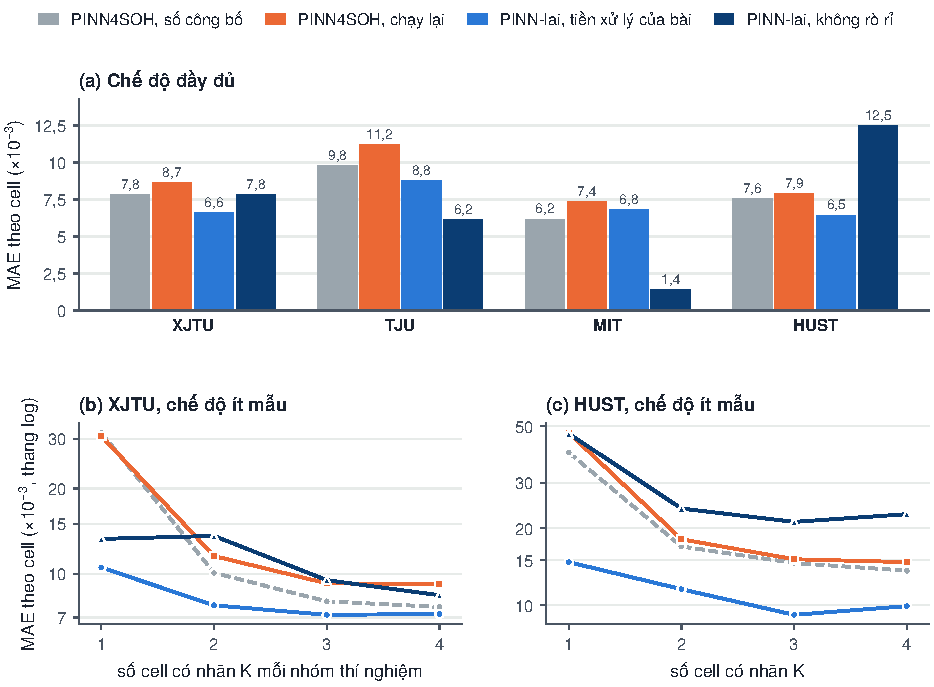
\includegraphics[width=\textwidth]{graphics/fig_benchmark.pdf}
\caption[So với PINN4SOH trên đúng cách chia của bài]{MAE theo cell trên đúng các nhóm đánh giá của bài PINN4SOH. (a) Chế độ đầy đủ, mỗi bộ bốn cột: số công bố của bài, mã gốc của bài chạy lại, PINN-lai với tiền xử lý của bài và PINN-lai với tiền xử lý không rò rỉ. (b), (c) Chế độ ít mẫu: MAE theo số cell có nhãn $K$.}\label{fig:bench}
\end{figure}

Theo RMSE, Bảng~\ref{tab:pubrmse} lấy trên mỗi bộ mô hình có sai số thấp nhất của đồ án và ghi tên mô hình đó. RMSE thấp nhất của đồ án thấp hơn số công bố ở XJTU, TJU và HUST (XJTU: PINN-lai, 22{,}2\,\%; TJU: PINN-lai, 14{,}0\,\%; HUST: PINN-lai, 16{,}3\,\%). Ở MIT, GBDT cao hơn 0{,}2\,\%.

\begin{table}[!htbp]\centering\small
\caption[RMSE tốt nhất của đồ án so với PINN4SOH]{RMSE ($\times10^{-3}$) trên đúng cách chia của bài PINN4SOH, chế độ đầy đủ, cùng tiền xử lý với bài. Cột thứ hai tính từ tệp kết quả công bố cùng mã nguồn của bài; cột thứ ba là RMSE thấp nhất trong PINN-lai, GBDT và PINN-semi của đồ án, cột Mô hình ghi mô hình đạt được. Cả hai cột lấy trung bình qua cell kiểm tra, lần chạy và nhóm như Bảng~\ref{tab:pub}. In đậm: thấp hơn trong hai cột. Chênh lệch là RMSE của đồ án so với số công bố, âm là đồ án thấp hơn.}\label{tab:pubrmse}
\begin{tabular}{lrrlr}\toprule
Bộ dữ liệu & RMSE PINN4SOH công bố $\downarrow$ & RMSE tốt nhất của đồ án $\downarrow$ & Mô hình & Chênh lệch $\downarrow$ \\\midrule
XJTU & 10{,}88 & \textbf{8{,}47} & PINN-lai & $-$22{,}2\,\% \\
TJU & 12{,}28 & \textbf{10{,}56} & PINN-lai & $-$14{,}0\,\% \\
MIT & \textbf{7{,}51} & 7{,}52 & GBDT & $+$0{,}2\,\% \\
HUST & 8{,}69 & \textbf{7{,}27} & PINN-lai & $-$16{,}3\,\% \\
\bottomrule\end{tabular}\end{table}

\subsection{Các chỉ số tốt hơn các bài báo đã công bố}
Cùng cách chia và cùng tiền xử lý với bài, PINN-lai có sai số thấp hơn mã gốc PINN4SOH chạy lại ở 12 trên 12 chế độ, thấp hơn có ý nghĩa thống kê ở 7 (tỉ số 0{,}76--0{,}92 ở chế độ đầy đủ, 0{,}31--0{,}79 ở chế độ ít mẫu) và không chế độ nào cao hơn có ý nghĩa thống kê (Bảng~\ref{tab:pub}). So với số công bố của PINN4SOH, PINN-lai thấp hơn ở 11 trên 12 chế độ (tỉ số 0{,}84--1{,}10 ở chế độ đầy đủ, 0{,}33--0{,}94 ở chế độ ít mẫu). Lợi thế lớn nhất ở chế độ ít mẫu, nơi hàm mất mát vật lý được tính cả trên các cell huấn luyện không nhãn. So với MLP và CNN mà bài PINN4SOH báo cáo, PINN-lai thấp hơn MLP ở 12 trên 12 chế độ và thấp hơn CNN ở 11 trên 12. Với tiền xử lý không rò rỉ, PINN-lai vẫn thấp hơn số công bố của PINN4SOH trên TJU (tỉ số 0{,}63), MIT (tỉ số 0{,}23), thấp hơn có ý nghĩa thống kê theo cell ở 2 trên 4 bộ đầy đủ, và ở XJTU $K = 1$ (tỉ số 0{,}42).

\subsection{Các chỉ số chưa tốt}
So với các bài báo đã công bố, đồ án còn một số điểm chưa đạt. Cùng điều kiện với bài, PINN-lai chưa thấp hơn số công bố của PINN4SOH ở MIT đầy đủ (6{,}80 so với 6{,}18), và chưa thấp hơn CNN của bài ở MIT đầy đủ (6{,}15). Một GBDT đơn giản với cùng tiền xử lý rò rỉ tốt ngang PINN-lai: tỉ số GBDT/PINN-lai 0{,}69--1{,}06, GBDT thấp hơn có ý nghĩa thống kê ở 2 chế độ (HUST $K = 1$, HUST $K = 2$) và không chế độ nào cao hơn. Với min--max theo cell, chỉ số chu kỳ đã chuẩn hoá là phần đời đã qua và mô hình cây khai thác thẳng thông tin này, nên lợi thế so với mã gốc trong điều kiện đó không thể quy cho phần vật lý. Với tiền xử lý không rò rỉ, PINN-lai cao hơn số công bố trên HUST (tỉ số 1{,}65), ngang trên XJTU (0{,}99), cao hơn có ý nghĩa thống kê theo cell ở 1 trên 4 bộ đầy đủ. Ở chế độ ít mẫu cao hơn ở 7 trên 8 (tỉ số 1{,}10--1{,}66). Đây là các chế độ mà tiền xử lý của bài có lợi nhiều nhất: khi chỉ có vài cell có nhãn, biết cell đã đi được bao nhiêu phần đời gần như là biết SOH. Đồ án không dùng tiền xử lý đó vì nó không thực hiện được khi triển khai (Mục~\ref{sec:dt_bo}). Đồ án không tái lập được chính xác số công bố của PINN4SOH: mã gốc chạy lại cho sai số bằng 1{,}04--1{,}19 lần ở chế độ đầy đủ, cao hơn có ý nghĩa thống kê theo cell ở 2 trên 4 bộ (Bảng~\ref{tab:pub}). Các hàng huấn luyện dựng lại trùng với dữ liệu của bài, nên phần chênh đến từ phần cứng và phiên bản thư viện.

Ngay trong các so sánh của chính đồ án, một số chỉ số cũng chưa đạt. GBDT đơn lẻ có sai số thấp hơn PINN-semi ở 14/16 trường hợp bộ $\times$ mức nhãn (10 có ý nghĩa thống kê). PINN-semi chỉ vượt GBDT có ý nghĩa thống kê ở HUST 30\,\% nhãn (Mục~\ref{sec:labels}). PINN-lai cố định vẫn kém GBDT có ý nghĩa thống kê ở TJU 70\,\%. Ở 70\,\% nhãn, PINN-semi kém MLP có ý nghĩa thống kê trên TJU (tỉ số 1{,}09). Với kiểm định bảo thủ ở mức fold, lợi ích ở 30\,\% nhãn chỉ đứng vững trên MIT. Khoảng dự đoán 90\,\% của ước lượng SOH có độ phủ thực tế 84{,}9--92{,}6\,\% (trung bình 88{,}8\,\%), 14--25\,\% số cell có độ phủ dưới 80\,\%. Với HiPINN (\Cref{sec:e33res}), khoảng SOH 90\,\% tính bằng phương pháp conformal phủ 89--93\,\% tuỳ bộ và ngân sách, khoảng RUL 90\,\% phủ 68--87\,\%. Tỉ lệ dự báo RUL nằm trong $\pm 20\,\%$ RUL thật là 53--84\,\%. Ở 10\,\% đời cuối của XJTU, MAE của HiPINN vẫn là 30{,}0 ($\times10^{-3}$). Tham số vật lý $\lambda$, $E_a$ không được dữ liệu xác định, và tốc độ $r$ học được thấp hơn nhiều tốc độ suy giảm thực đo (\Cref{sec:vatly}). Bộ lọc xu thế không bảo đảm SOH dự đoán không tăng (đầu ra tăng ở 28--44\,\% số bước). Ép không tăng làm sai số trên XJTU tăng 1{,}76--1{,}94 lần vì dung lượng đo được của XJTU tăng ở đầu đời.

\subsection{Vai trò của phần vật lý}\label{sec:vatly}
Đề tài nhấn mạnh sự hỗ trợ của thông tin hoá lý, nên cần nói rõ phần vật lý trong PINN-semi thực sự đóng góp gì. Ba quan sát ở các mục trước cho thấy đóng góp này hẹp hơn tên gọi. Thứ nhất, chỉ riêng ràng buộc đơn điệu đã mang lại 62--95\,\% mức giảm sai số của PINN-semi so với MLP ở 30\,\% nhãn, còn bỏ phần dư động học và ràng buộc miền chỉ làm MAE tăng 1--11\,\% (\Cref{sec:source}). Thứ hai, các tham số hoá lý dịch chuyển ít so với giá trị khởi tạo: $\lambda$ (khởi tạo bằng 1) của các PINN-semi nằm trong khoảng 0{,}96--0{,}98 ở XJTU, 0{,}95--0{,}97 ở TJU, 0{,}95--0{,}97 ở MIT và 0{,}90--1{,}26 ở HUST, còn $E_a$ khởi tạo ở 30\,kJ/mol thì dịch không quá 1{,}6\,kJ/mol. Thứ ba, tốc độ $r$ học được trung bình chỉ 0{,}001--0{,}063, trong khi tốc độ suy giảm thực đo là 0{,}137--0{,}356 SOH trên 1\,000 chu kỳ. Cả ba có nguyên nhân trong cách đặt bài toán, không phải do tối ưu chưa hội tụ.

Phần dư động học ràng buộc đạo hàm riêng $\partial u/\partial t$ khi giữ nguyên đặc trưng sạc. Trên quỹ đạo thật của một cell, SOH thay đổi chủ yếu vì đặc trưng sạc thay đổi theo tuổi, tức qua số hạng $\nabla_{\mathbf{x}} u \cdot \mathrm{d}\mathbf{x}/\mathrm{d}n$, còn $t$ chỉ là một trong 17 đầu vào. Mạng nghiệm vì vậy thoả được phương trình với một đạo hàm riêng nhỏ theo $t$, và $r$ học được nhỏ hơn nhiều so với tốc độ suy giảm thật. Với trọng số $\alpha = 0{,}02$, phần dư này chủ yếu buộc đạo hàm theo $t$ không dương, điều mà ràng buộc đơn điệu đã làm trực tiếp hơn.

Hệ số $\lambda$ khó xác định vì thừa số $g(u) = e^{\lambda(1-u)}$ chỉ thay đổi khoảng 22\,\% khi SOH đi từ 1 xuống 0,8 với $\lambda \approx 1$. Sự phụ thuộc vào mức suy giảm này đã có sẵn trong $k(\tilde{\mathbf{x}})$, vốn nhận các đặc trưng sạc biến thiên theo tuổi. Hai thừa số thay thế được cho nhau, nên dữ liệu chỉ kéo $\lambda$ đi một đoạn ngắn khỏi giá trị khởi tạo, xa nhất ở HUST.

Năng lượng hoạt hoá $E_a$ thì không định danh được về mặt toán học trên ba bộ. Thừa số Arrhenius $A(T) = \exp[-(E_a/R_g)(1/T - 1/T_\text{ref})]$ chỉ khác 1 khi nhiệt độ khác $T_\text{ref}$. Ở XJTU, mọi cell chạy ở 298{,}15\,K, đúng bằng $T_\text{ref}$, nên $1/T - 1/T_\text{ref} = 0$, $A \equiv 1$ và gradient của hàm mất mát theo $E_a$ bằng 0. Thực tế $E_a$ của mọi PINN-semi trên XJTU giữ đúng 30{,}0\,kJ/mol. Ở MIT và HUST, nhiệt độ là hằng 303{,}15\,K, nên $A$ chỉ là một hằng số nhân và bị $k(\tilde{\mathbf{x}}) = \operatorname{softplus}(G_\theta(\tilde{\mathbf{x}}))$ hấp thụ: mọi giá trị $E_a$ cho cùng một $r$ nếu $G_\theta$ bù lại. Chỉ TJU có ba mức nhiệt độ (298{,}15, 308{,}15 và 318{,}15\,K), nơi $E_a$ về nguyên tắc định danh được. Nhưng ở đó nhiệt độ chỉ làm sai số thay đổi dưới 1\,\% (thêm $1/T$ vào GBDT cho tỉ số 0{,}99--1{,}00, \Cref{sec:dt_bo}), nên dữ liệu cũng không đủ để ước lượng $E_a$ chính xác.

Dù vậy, phần vật lý vẫn có giá trị ở ba điểm. Một là ràng buộc đơn điệu và ràng buộc miền là tiên nghiệm vật lý đúng, và chúng được áp lên cả cell không nhãn. Ở 10\,\% nhãn, phần lợi ích do áp hàm mất mát vật lý lên cell không nhãn (PINN-semi so với PINN-sup, tỉ số 0{,}62--0{,}94) chiếm 50--64\,\% mức giảm sai số so với MLP. Hai là dạng tốc độ có cấu trúc, luôn không âm, ngăn lời giải tầm thường $G \approx u_t$ của động học hộp đen kiểu PINN4SOH, nên các ràng buộc thực sự tác động lên mạng nghiệm. Ba là ở bài toán dự báo, nghiệm đóng của cùng động học xám cho PINN-dự báo một đường ngoại suy có dạng vật lý: luôn không tăng, có thể gãy dần hoặc chậm dần, với chỉ hai tham số. PINN-dự báo là một trong ba nhánh của HiPINN. Vì vậy cụm “thông tin hoá lý” trong đồ án nên được hiểu là các tiên nghiệm có cấu trúc (đơn điệu, miền giá trị, tốc độ không âm, dạng Arrhenius, dạng nghiệm đóng), chứ không phải việc xác định các tham số điện hoá của cell.

\subsection{Nhận xét}
Trên đúng cách chia của PINN4SOH và cùng cách tính sai số, PINN-lai của đồ án có sai số thấp hơn số công bố ở phần lớn các chế độ và thấp hơn mã gốc chạy lại ở mọi chế độ. Tuy vậy, trong điều kiện có rò rỉ của bài, một GBDT cũng đạt kết quả tương tự, còn khi bỏ rò rỉ thì hơn hay kém tuỳ bộ dữ liệu. Vì thế, những đóng góp có cơ sở vững nhất của đồ án là giao thức đánh giá không rò rỉ, các so sánh ghép cặp có kiểm định trong cùng một giao thức, và các mô hình có đặc trưng lịch sử HiGBDT, HiPINN cho bài toán dự báo.

